%% Multi-FPGA Distributed Quantum Circuit Simulation
%% Author: Nasir Ali, C-DAC Noida

\documentclass[pdflatex,sn-mathphys-num]{sn-jnl}
\pdfgentounicode=1
\input{glyphtounicode}
\usepackage[T1]{fontenc}
\usepackage{lmodern}
\usepackage{graphicx}
\usepackage{multirow}
\usepackage{amsmath,amssymb,amsfonts}
\usepackage{amsthm}
\usepackage[title]{appendix}
\usepackage{xcolor}
\usepackage{textcomp}
\usepackage{manyfoot}
\usepackage{booktabs}
\usepackage[utf8]{inputenc}
\usepackage{algorithm}
\usepackage{algorithmicx}
\usepackage{algpseudocode}
\usepackage{array}
\newcommand{\ket}[1]{\lvert #1\rangle}
\usepackage{url}

% bitwise operators as explicit math symbols (they survive text extraction of the PDF)
\newcommand{\band}{\mathbin{\&}}
\newcommand{\bor}{\mathbin{|}}
\newcommand{\shr}{\mathbin{\gg}}
\newcommand{\shl}{\mathbin{\ll}}

\newcommand{\NumAblGhzFourAllOff}{4.1}
\newcommand{\NumAblGhzFourFoneOff}{1.05}
\newcommand{\NumAblGhzFourFtwoOff}{1.9}
\newcommand{\NumAblGhzFourN}{28}
\newcommand{\NumAblGhzTwoAllOff}{2.8}
\newcommand{\NumAblGhzTwoFoneOff}{0.99}
\newcommand{\NumAblGhzTwoFtwoOff}{1.8}
\newcommand{\NumAblGhzTwoN}{28}
\newcommand{\NumAblGroverFourAllOff}{55.5}
\newcommand{\NumAblGroverFourFoneOff}{1.02}
\newcommand{\NumAblGroverFourFtwoOff}{101.8}
\newcommand{\NumAblGroverFourN}{14}
\newcommand{\NumAblGroverTwoAllOff}{59.0}
\newcommand{\NumAblGroverTwoFoneOff}{1.06}
\newcommand{\NumAblGroverTwoFtwoOff}{108.8}
\newcommand{\NumAblGroverTwoN}{14}
\newcommand{\NumAblPhFourAllOff}{1.0}
\newcommand{\NumAblPhFourFoneOff}{1.01}
\newcommand{\NumAblPhFourFtwoOff}{1.0}
\newcommand{\NumAblPhFourN}{28}
\newcommand{\NumAblPhTwoAllOff}{1.0}
\newcommand{\NumAblPhTwoFoneOff}{1.02}
\newcommand{\NumAblPhTwoFtwoOff}{1.0}
\newcommand{\NumAblPhTwoN}{28}
\newcommand{\NumAblQftFourAllOff}{10.5}
\newcommand{\NumAblQftFourFoneOff}{1.26}
\newcommand{\NumAblQftFourFtwoOff}{9.2}
\newcommand{\NumAblQftFourN}{28}
\newcommand{\NumAblQftTwoAllOff}{6.3}
\newcommand{\NumAblQftTwoFoneOff}{1.13}
\newcommand{\NumAblQftTwoFtwoOff}{5.9}
\newcommand{\NumAblQftTwoN}{28}
\newcommand{\NumAblRandFourAllOff}{1.0}
\newcommand{\NumAblRandFourFoneOff}{0.99}
\newcommand{\NumAblRandFourFtwoOff}{1.0}
\newcommand{\NumAblRandFourN}{28}
\newcommand{\NumAblRandTwoAllOff}{1.0}
\newcommand{\NumAblRandTwoFoneOff}{0.99}
\newcommand{\NumAblRandTwoFtwoOff}{1.0}
\newcommand{\NumAblRandTwoN}{28}
\newcommand{\NumBarrierUs}{374}
\newcommand{\NumBaselineErrMax}{$1.38\times 10^{-7}$}
\newcommand{\NumBaselineExactErrMax}{$1.11\times 10^{-16}$}
\newcommand{\NumBaselineRotErrMax}{$1.38\times 10^{-7}$}
\newcommand{\NumBaselineRotErrMin}{$3.50\times 10^{-18}$}
\newcommand{\NumBramPctFlagship}{40.1}
\newcommand{\NumBramPctVsix}{11.8}
\newcommand{\NumClockFlagship}{300}
\newcommand{\NumClockVsix}{258}
\newcommand{\NumCorrectnessExact}{29}
\newcommand{\NumCorrectnessHaar}{43}
\newcommand{\NumCorrectnessInstances}{166}
\newcommand{\NumCorrectnessNmax}{31}
\newcommand{\NumCorrectnessNmin}{4}
\newcommand{\NumCpuAerFaster}{35}
\newcommand{\NumCpuAerOneCases}{37}
\newcommand{\NumCpuAerOneOverGhz}{36}
\newcommand{\NumCpuAerOneOverGroverSixteen}{0}
\newcommand{\NumCpuAerOneOverQft}{38}
\newcommand{\NumCpuAerOneOverQftSixteen}{0}
\newcommand{\NumCpuCases}{37}
\newcommand{\NumCpuFasterThanAerOne}{22}
\newcommand{\NumCpuFpgaFaster}{2}
\newcommand{\NumCpuRatioGhz}{1.3}
\newcommand{\NumCpuRatioGroverSixteen}{35.3}
\newcommand{\NumCpuRatioQft}{1.8}
\newcommand{\NumCpuRatioQftSixteen}{8.3}
\newcommand{\NumCpuWideCases}{14}
\newcommand{\NumCpuWideFasterThanAerOne}{14}
\newcommand{\NumDiagBarrierOffTwenty}{0.93}
\newcommand{\NumDiagBarrierOnTwenty}{0.12}
\newcommand{\NumDiagHostOffTwenty}{0.95}
\newcommand{\NumDiagHostOnTwenty}{0.34}
\newcommand{\NumDiagPcieTwenty}{1344}
\newcommand{\NumDiagSpeedupMax}{1.13}
\newcommand{\NumDiagSpeedupMin}{1.01}
\newcommand{\NumDiagSpeedupTwenty}{1.01}
\newcommand{\NumDspPctFlagship}{29.8}
\newcommand{\NumDspPctVsix}{8.1}
\newcommand{\NumEnergyIdleFour}{92}
\newcommand{\NumEnergyIdleOne}{33}
\newcommand{\NumEnergyIdleTwo}{66}
\newcommand{\NumEnergyPowerMaxFour}{145}
\newcommand{\NumEnergyPowerMaxOne}{45}
\newcommand{\NumEnergyPowerMaxTwo}{77}
\newcommand{\NumEnergyPowerMinFour}{137}
\newcommand{\NumEnergyPowerMinOne}{34}
\newcommand{\NumEnergyPowerMinTwo}{68}
\newcommand{\NumEnergyQftTwentyEightFour}{1072}
\newcommand{\NumEnergyQftTwentyEightOne}{482}
\newcommand{\NumEnergyQftTwentyEightTwo}{580}
\newcommand{\NumEnginesFlagship}{8}
\newcommand{\NumGhzChainRemapsFfour}{1}
\newcommand{\NumGhzChainRemapsFfourAll}{1}
\newcommand{\NumGhzChainRemapsNoFfour}{5}
\newcommand{\NumGhzChainSpeedupFfour}{4.0}
\newcommand{\NumGhzChainTimeFfour}{1.95}
\newcommand{\NumGhzChainTimeNoFfour}{7.85}
\newcommand{\NumGhzLogRemapsFfour}{3}
\newcommand{\NumGhzLogRemapsFfourAll}{4}
\newcommand{\NumGhzLogRemapsNoFfour}{5}
\newcommand{\NumGhzLogSpeedupFfour}{1.2}
\newcommand{\NumGhzLogTimeFfour}{7.63}
\newcommand{\NumGhzLogTimeNoFfour}{9.25}
\newcommand{\NumGhzTopRemapsFfourAll}{2}
\newcommand{\NumGhzTopSpeedupFfour}{2.3}
\newcommand{\NumGhzTopTimeFfour}{2.7}
\newcommand{\NumGhzTopTimeNoFfour}{6.18}
\newcommand{\NumGovernor}{ondemand}
\newcommand{\NumGroverSixteenExchPct}{57}
\newcommand{\NumGroverSixteenIters}{201}
\newcommand{\NumGroverSixteenRemaps}{2{,}417}
\newcommand{\NumGroverWorstPdiff}{$1.31\times 10^{-12}$}
\newcommand{\NumHbmAllCards}{379}
\newcommand{\NumHbmLmax}{24}
\newcommand{\NumHbmPerCard}{95}
\newcommand{\NumHbmPortsFlagship}{16}
\newcommand{\NumHostCores}{128}
\newcommand{\NumHostCoresMax}{256}
\newcommand{\NumHostCoresMin}{4}
\newcommand{\NumHostRamGiB}{503}
\newcommand{\NumHostRevisedQftTwenty}{0.157}
\newcommand{\NumHostSockets}{2}
\newcommand{\NumHostSpreadBaselinePct}{2}
\newcommand{\NumHostSpreadEnginePct}{21}
\newcommand{\NumHostSubmittedQftTwenty}{89.3}
\newcommand{\NumHostThreads}{256}
\newcommand{\NumLaunchMs}{0.8}
\newcommand{\NumLutPctFlagship}{37.3}
\newcommand{\NumLutPctVsix}{16.1}
\newcommand{\NumMaxThirtyOneGhzS}{13.7}
\newcommand{\NumMaxThirtyOneGhzVerified}{yes}
\newcommand{\NumMaxThirtyOneQftS}{60.8}
\newcommand{\NumMaxThirtyOneQftVerified}{yes}
\newcommand{\NumMaxWidthFourCards}{31}
\newcommand{\NumMaxWidthOneCard}{29}
\newcommand{\NumMaxWidthTwoCards}{30}
\newcommand{\NumModelCrossN}{12}
\newcommand{\NumModelNstarMax}{11.0}
\newcommand{\NumModelNstarMin}{9.9}
\newcommand{\NumModelRatioMax}{1.09}
\newcommand{\NumModelRatioMin}{0.96}
\newcommand{\NumModelSweepShareEight}{3}
\newcommand{\NumOpCostModelMs}{3.50}
\newcommand{\NumOpCostMs}{3.78}
\newcommand{\NumPartRatioMax}{1.73}
\newcommand{\NumPartRatioMin}{0.69}
\newcommand{\NumPassmL}{22}
\newcommand{\NumPcsPerEngineFlagship}{4}
\newcommand{\NumPcsUsedFlagship}{32}
\newcommand{\NumQftTwentyEightKernelPct}{41}
\newcommand{\NumQftTwentyEightPciePct}{55}
\newcommand{\NumQftTwentyEightSpeedupFour}{1.77}
\newcommand{\NumQftTwentyEightSpeedupTwo}{1.62}
\newcommand{\NumQpeWorstDistDiff}{$8.88\times 10^{-15}$}
\newcommand{\NumQueueRttUs}{359}
\newcommand{\NumRefSvMax}{20}
\newcommand{\NumRepsMax}{11}
\newcommand{\NumRepsMin}{1}
\newcommand{\NumRouteQftExch}{9}
\newcommand{\NumRouteQftFone}{44}
\newcommand{\NumRouteQftFtwo}{85}
\newcommand{\NumRouteQftGates}{420}
\newcommand{\NumRouteQftLocal}{268}
\newcommand{\NumRouteQftPasses}{76}
\newcommand{\NumScaleBelowOne}{21}
\newcommand{\NumScaleBestFour}{1.77}
\newcommand{\NumScaleBestFourN}{28}
\newcommand{\NumScaleCases}{32}
\newcommand{\NumScaleExchDevQftFour}{0.176}
\newcommand{\NumScaleExchDevQftOne}{0.838}
\newcommand{\NumScaleExchDevRandFour}{0.39}
\newcommand{\NumScaleExchDevRandOne}{1.09}
\newcommand{\NumScaleExchHostQftFour}{3.45}
\newcommand{\NumScaleExchHostQftOne}{0}
\newcommand{\NumScaleExchHostRandFour}{14.9}
\newcommand{\NumScaleExchHostRandOne}{7.03}
\newcommand{\NumScaleExchQftFour}{47}
\newcommand{\NumScaleExchQftOne}{6}
\newcommand{\NumScaleExchRandFour}{78}
\newcommand{\NumScaleExchRandOne}{37}
\newcommand{\NumSubmittedOverRevisedQftTwenty}{569}
\newcommand{\NumThermalStops}{7}
\newcommand{\NumUramPctFlagship}{6.7}
\newcommand{\NumVsixCyclesPerAmp}{85}
\newcommand{\NumVsixLaunchMsSixteen}{0.14}
\newcommand{\NumVsixLaunchMsTen}{0.13}
\newcommand{\NumVsixNsPerAmp}{329}
\newcommand{\NumVsixPhTwentyTwoHostPct}{26}
\newcommand{\NumVsixPhTwentyTwoKernelPct}{0}
\newcommand{\NumVsixPhTwentyTwoPciePct}{48}
\newcommand{\NumVsixPhTwentyTwoSyncPct}{27}
\newcommand{\NumVsixQftEightHostPct}{3}
\newcommand{\NumVsixQftEightKernelPct}{12}
\newcommand{\NumVsixQftEightPciePct}{32}
\newcommand{\NumVsixQftEightSyncPct}{54}
\newcommand{\NumVsixQftTwentyTwoHostPct}{0}
\newcommand{\NumVsixQftTwentyTwoKernelPct}{98}
\newcommand{\NumVsixQftTwentyTwoPciePct}{1}
\newcommand{\NumVsixQftTwentyTwoSyncPct}{1}
\newcommand{\NumVsixSweepMsSixteen}{21.56}
\newcommand{\NumVsixSweepMsTen}{0.35}
\newcommand{\NumVsixXferMsTen}{0.49}
\newcommand{\NumWeakEffFourMax}{45}
\newcommand{\NumWeakEffFourMin}{20}
\newcommand{\NumWorstMaxAbsErr}{$2.00\times 10^{-13}$}
\newcommand{\NumWorstOneMinusF}{$8.07\times 10^{-25}$}

\theoremstyle{thmstyleone}
\newtheorem{theorem}{Theorem}
\theoremstyle{thmstylethree}
\newtheorem{definition}{Definition}

\raggedbottom

\begin{document}

\title[Multi-FPGA Quantum Circuit Simulation]{Multi-FPGA Quantum Circuit Simulation: A Distributed Statevector Architecture on Four Xilinx Alveo U55C Accelerators}

\author*[1]{\fnm{Nasir} \sur{Ali}}\email{nasirali2607@gmail.com}

\affil*[1]{\orgdiv{Embedded Systems Division},
           \orgname{Centre for Development of Advanced Computing},
           \orgaddress{\city{Noida}, \postcode{201307}, \country{India}}}

\abstract{Exact statevector simulation of quantum circuits needs memory that doubles with every qubit. We distribute a complex128
statevector over the high bandwidth memory of one, two or four AMD Alveo U55C cards in one host and evaluate the design
on the physical cards. A single primitive, a $2\times2$ complex128 matrix applied to amplitude pairs under a per
operation slice enable, lets the cards execute every gate that needs no amplitudes of another card, including diagonal,
controlled and permutation gates on the partition qubits and wide multi controlled gates, while a compiler packs gates
into passes over memory and moves amplitudes only for the remaining gates. Each card runs \NumEnginesFlagship~engines, which use all \NumPcsUsedFlagship~memory
channels of the card. The system simulates \NumMaxWidthOneCard~qubits on one card, \NumMaxWidthTwoCards~on two and \NumMaxWidthFourCards~on four cards,
the largest widths its memory layout allows; all \NumCorrectnessInstances~checked instances agree with an independent reference to double precision rounding.
On the same cards the quantum Fourier transform at 20 qubits runs \NumSubmittedOverRevisedQftTwenty~times faster than
in a baseline design that computes the gates on partition qubits on the host, whose timing a microbenchmark model reproduces without fitted parameters. Ablations, timing
breakdowns, scaling, energy and host measurements show where the time goes: distribution adds capacity, not speed,
because exchanges between cards pass through host memory, and Qiskit Aer on the \NumHostCores~core host is faster for almost all
circuits measured.}

\keywords{Multi-FPGA, Quantum circuit simulation, Distributed statevector, HBM2, Alveo U55C, Quantum Fourier transform,
Complex128 precision}

\maketitle

\section{Introduction}\label{sec:introduction}

Classical simulation of quantum circuits remains essential for algorithm development, compiler verification and
the validation of quantum hardware~\cite{preskill2018nisq,arute2019supremacy}. Exact statevector simulation stores all
$2^n$ complex amplitudes of an $n$ qubit register; in complex128 (16~bytes per amplitude) this is 4~GiB at $n=28$, 16~GiB
at $n=30$ and 64~GiB at $n=32$, so that every additional qubit doubles both memory and work. Distributing the state
over several devices is the established way to go beyond one device, both on CPU clusters and on
GPUs~\cite{smelyanskiy2016qhipster,jones2019quest,haner2017petabyte,deraedt2019massively,imamura2022mpiqulacs,bayraktar2023cuquantum}.
On FPGAs, statevector designs have mostly targeted one device~\cite{khalid2004fpga,lee2016fpga,pilch2019fpga,mahmud2019scaling,pcq2024,tiwari2026fpga30};
the Trefoil system distributes very large state vectors over several FPGAs backed by SATA disk arrays~\cite{niwase2023trefoil,wei2025qutrefoil}.

This paper studies a different point of that design space: a statevector held entirely in the high bandwidth memory
of four AMD Alveo U55C cards in one host, with complex128 arithmetic throughout. It is the multi card continuation of
the single card complex64 simulator of the companion paper~\cite{tiwari2026fpga30}, which reaches 30 qubits on one card
and contains the comparison of that design with CPU and GPU simulators. We compare two ways of dividing the work
between host and cards. In a baseline design, one kernel per card applies the local gates while every gate on a
partition qubit is computed on the host after the card's whole slice has been moved over PCIe. Our engine instead
executes every gate that does not need another card's amplitudes inside the FPGA, including diagonal and controlled
gates on partition qubits, and moves data only for the remaining gates.

The contributions, each supported by measurements on the four cards, are:
\begin{enumerate}
\item A complex128 statevector engine for the U55C with one compute unit per group of HBM pseudo channels, built
around a single $2\times2$ multiplexed primitive with a per operation slice enable, and a host runtime that distributes
the state over one, two or four cards. The engine holds \NumMaxWidthOneCard~qubits on one card and
\NumMaxWidthFourCards~qubits on four cards, verified amplitude by amplitude against an independent reference
(Section~\ref{subsec:res-correctness}).
\item Execution of diagonal, partition controlled and partition permutation gates without data movement (F1 to F3),
and a hardware specific compiler rewrite for $X$ type gates on partition qubits (F4). Ablations quantify each of
them (Section~\ref{subsec:res-ablation}).
\item A measured account of where the time goes: per phase timing, bytes moved over PCIe, scaling over one, two and
four cards, the sensitivity to the host, the board energy, and a model of the baseline design built only from
microbenchmarks that explains its timing curve (Sections~\ref{subsec:res-breakdown} to~\ref{subsec:res-model}).
\item An honest comparison with Qiskit on the same host and the same circuits (Section~\ref{subsec:res-cpu}).
\end{enumerate}
We make no claim that the FPGA system outperforms CPU or GPU statevector simulators. Section~\ref{subsec:res-cpu} shows
where Qiskit Aer on the \NumHostCores~core host is faster and where it is not; the GPU comparison of the same card type is
reported in the companion paper~\cite{tiwari2026fpga30}.
\section{Related Work}\label{sec:related}

\subsection{Distributed statevector simulation on CPUs and GPUs}\label{subsec:related-dist}

Exact statevector simulation beyond the memory of one node distributes the $2^n$ amplitudes over many processes,
each holding a contiguous slice selected by the top qubits, and exchanges amplitudes when a gate acts on such a global
qubit. qHiPSTER, later the Intel Quantum Simulator, combined vectorisation, multithreading, cache blocking and
overlap of computation with communication and simulated circuits of up to 40 qubits on a supercomputer, limited by
memory and network bandwidth~\cite{smelyanskiy2016qhipster,guerreschi2020intel}. QuEST is a hybrid multithreaded,
distributed and GPU accelerated simulator that benchmarked random circuits of up to 38 qubits on up to 2048 nodes~\cite{jones2019quest}.
H\"aner and Steiger used generated and optimised kernels and a scheduling algorithm that reduces communication to
simulate a 45 qubit circuit on 8192 nodes~\cite{haner2017petabyte}; the J\"ulich simulator reached 48 qubits with an
adaptive encoding of the wave function and showed close to ideal weak scaling on several supercomputers~\cite{deraedt2019massively};
mpiQulacs is a distributed statevector simulator optimised for A64FX clusters~\cite{imamura2022mpiqulacs}. On GPUs,
HyQuas selects among partitioning methods per circuit pattern to improve data locality~\cite{zhang2021hyquas}, and the
cuQuantum SDK provides composable GPU primitives for quantum circuit simulation~\cite{bayraktar2023cuquantum};
Qulacs is a widely used single node CPU and GPU simulator~\cite{suzuki2021qulacs}. Simulations at 49 qubits and beyond
rely on other representations, such as tensor network contraction and low depth circuit
structure~\cite{markov2008simulating,pednault2017breaking,chen2018sixtyfour,boixo2018characterizing,villalonga2019flexible}.

Two techniques of these systems are central to the present work. First, a gate that is diagonal in the computational
basis never needs amplitudes of another process, even when it acts on a global qubit, and a gate controlled by a
global qubit acts only on the processes whose bit is one; second, global and local qubits can be swapped once so that
a sequence of gates on a global qubit runs locally (global to local remapping), and gates can be scheduled to reduce
the number of such exchanges~\cite{haner2017petabyte}. Executing diagonal gates on partition qubits without exchange is the
first technique; it is not new as an algorithmic idea, and we do not claim it as such. What this paper contributes is the
implementation of these techniques inside FPGA kernels: the slice enable lets every card's HBM engines execute
partition diagonal, partition controlled and partition permutation gates in their streaming passes without host
arithmetic or PCIe traffic, and remaps run as device copies inside a card and as half slice exchanges across cards.

\subsection{FPGA statevector simulators}\label{subsec:related-fpga}

FPGA emulation of quantum circuits was proposed by Khalid, Zilic and Radecka~\cite{khalid2004fpga}. Lee et al.\
presented a serial parallel FPGA emulation architecture with the QFT and Grover's search as case studies and a linear
reduction of resources compared with pipelined designs~\cite{lee2016fpga}; Pilch and D\l{}ugopolski proposed a
universal FPGA emulator with a standard programming interface~\cite{pilch2019fpga}; Mahmud, El-Araby and Caliga
studied scalable reconfigurable emulation at high precision and throughput~\cite{mahmud2019scaling}. More recent work
includes Q2Logic, a coarse grained reconfigurable overlay specialised for Schr\"odinger style
simulation~\cite{podobas2023q2logic}, PCQ, a parallel pipelined dataflow architecture with data decoupling that
partitions computation into non interacting subsets~\cite{pcq2024}, and a scalable accelerator architecture that
addresses parallelism and the routing of state components~\cite{belfore2024scalable}. These designs target one
device. Statevector simulation over several FPGAs has been demonstrated by the Trefoil system, which combines
multiple FPGAs with SATA disk arrays (2~PB of storage in eight storage subsystems) to hold state vectors of up to 47
qubits, at the cost of disk bandwidth (an H gate on 30 qubits takes about 10 minutes)~\cite{niwase2023trefoil}; its
simulator, Qu-Trefoil, builds on this storage based platform~\cite{wei2025qutrefoil}. The present work takes the
opposite design point: the whole state stays in the HBM of the cards and moves over PCIe only when a gate requires
amplitudes of another card, which limits the width to what the HBM of the cards holds but keeps every gate at HBM
bandwidth. The companion paper of this work~\cite{tiwari2026fpga30} reaches 30 qubits in complex64 on one U55C with HBM and
compares it with CPU and GPU simulators; the present paper is the multi card, complex128 continuation that the
companion paper names as future work. Further related designs of the author on the same platform, a native RTL
statevector engine in FP64~\cite{ali2026rtl}, real time error correction decoders~\cite{ali2026qec} and a matrix
product state engine~\cite{ali2026mps}, are available as preprints.
\section{System Architecture}\label{sec:architecture}

\subsection{Hardware platform}\label{subsec:hw}

The system is a single host server with four AMD (Xilinx) Alveo U55C accelerator cards on PCIe Gen3 x16
(Table~\ref{tab:platform}). Each card carries the XCU55C device and 16~GiB of HBM2 organised as 32 pseudo channels
(PCs) of 512~MiB; every HBM AXI port of a kernel reaches any PC through the HBM switch~\cite{amd_ds978,amd_ug1393}.
Device capacities in Table~\ref{tab:platform} are those of the data sheet~\cite{amd_ds978}; utilisation, achieved
clock and PC bindings are taken from the post route reports of the bitstreams used here (Section~\ref{subsec:res-resources}).
The host has \NumHostCores~cores in \NumHostSockets~sockets and \NumHostRamGiB~GiB of memory; three cards are attached
to NUMA node~0 and one to node~1 (Section~\ref{subsec:res-host}).

\begin{table}[t]
\caption{Platform. Device values from the AMD U55C data sheet~\cite{amd_ds978}; host values captured by script at
measurement time (\texttt{results/hardware\_manifest.json}).}\label{tab:platform}
\begin{tabular}{@{}ll@{}}
\toprule
FPGA device & AMD XCU55C on Alveo U55C (4 cards, shell xilinx\_u55c\_gen3x16\_xdma\_base\_3) \\
HBM2 per card & 16 GiB in 32 pseudo channels of 512 MiB \\
Host CPU & 2 $\times$ AMD EPYC 7742 64-Core Processor, 128 cores, 256 threads \\
Host memory & 503 GiB \\
Card NUMA nodes & 01: 0, 21: 0, 41: 0, a1: 1 \\
OS, XRT, Vitis & Ubuntu 20.04.6 LTS (5.15.0-139-generic), XRT 2.16.204, Vitis 2023.2 \\
Python stack & Python 3.8.20, NumPy 1.24.4, Qiskit 1.2.4, Qiskit Aer 0.15.1 \\
\bottomrule
\end{tabular}
\end{table}

\subsection{Distribution of the statevector}\label{subsec:partition}

An $n$ qubit state of $2^n$ complex128 amplitudes (16~bytes each) is split into $S = C\,P$ \emph{slices} of $2^L$
amplitudes, $L = n - \log_2 S$, where $C \in \{1,2,4\}$ is the number of cards and $P$ the number of slices per card.
Physical qubits $0,\dots,L-1$ are local to a slice; the next $\log_2 P$ physical qubits select the slice inside a card
and the top $\log_2 C$ select the card. Card $j$ therefore holds every amplitude whose top $\log_2 C$ index bits
equal $j$, and each card divides its share into $P$ slices, each stored in one HBM buffer (Section~\ref{subsec:engine}). We call the
$\log_2 S$ qubits above $L$ the \emph{slice qubits}; the top $\log_2 C$ of them are the \emph{partition qubits}. Capacities follow directly: an $n$ qubit complex128 state needs $2^{n+4}$~bytes, i.e.\ 16~MiB at
$n=20$, 4~GiB at $n=28$, 8~GiB at $n=29$ and 16~GiB at $n=30$, so that four cards (64~GiB in total) can hold
up to $n = 31$ when the state uses all PCs (Section~\ref{subsec:res-maxwidth} explains why not $n=32$).

\subsection{Baseline design}\label{subsec:baseline-design}

The single card design of the companion paper~\cite{tiwari2026fpga30} uses sixteen HBM data ports in complex64. When the
datapath was widened to complex128 for this work, the sixteen port kernel no longer routed: the implementation failed
with routing congestion and no bitstream was produced. The data ports were therefore halved, which gives the baseline
kernel. Each data bank needs its own AXI port and the gate sequence one more, so the design could not simply
spread the state over all 32 PCs. The baseline design thus uses one compute unit per card with eight HBM data ports and one gate buffer port,
bound to HBM[0] to HBM[7] and HBM[8]; amplitude $i$ of a card's slice is stored in port $i \bmod 8$, so each card
addresses nine PCs (4.5~GiB) of its 16~GiB. The kernel implements the 19 opcodes of Table~\ref{tab:opcodes} in
complex128 arithmetic; gate angles are transferred as float32 and widened in the kernel. With $n_\ell = n - \log_2 C$
local qubits, a single qubit gate on local qubit $q$ visits the $2^{n_\ell-1}$ amplitude pairs
\begin{equation}
i_0 = \bigl((k \shr q) \shl (q+1)\bigr) \bor \bigl(k \band (2^q-1)\bigr), \qquad i_1 = i_0 + 2^q,
\qquad k = 0,\dots,2^{n_\ell-1}-1, \label{eq:pair}
\end{equation}
and applies the $2\times2$ gate matrix to $(\alpha_{i_0}, \alpha_{i_1})$. CX with control $c$ and target $t$ swaps
$\alpha_i$ and $\alpha_{i \oplus 2^t}$ for every $i$ with $(i \band 2^c) \ne 0$ and $(i \band 2^t) = 0$; CZ negates
\begin{equation}
\alpha_i \leftarrow -\alpha_i \quad \text{for every } i \text{ with } (i \band 2^c) \ne 0 \text{ and } (i \band 2^t) \ne 0.
\label{eq:cz}
\end{equation}
A controlled phase $\mathrm{CP}(\theta)$ whose control is partition bit $p_b$ of card index $j$ and whose target is
local qubit $q_t$ changes only amplitudes of the card itself:
\begin{equation}
\alpha_i' = \begin{cases} e^{i\theta}\,\alpha_i & \text{if } \bigl((j \shr p_b) \band 1\bigr) = 1 \text{ and }
\bigl((i \shr q_t) \band 1\bigr) = 1,\\ \alpha_i & \text{otherwise.}\end{cases} \label{eq:diag}
\end{equation}

\begin{table}[t]
\caption{Opcodes of the baseline kernel (19, complex128 arithmetic), as defined in its source.}\label{tab:opcodes}
\begin{tabular}{@{}rlrlrlrl@{}}
\toprule
Opcode & Gate & Opcode & Gate & Opcode & Gate & Opcode & Gate \\
\midrule
0 & I & 5 & $S$ & 10 & $\sqrt{X}^\dagger$ & 15 & $U_2(\phi,\lambda)$ \\
1 & $H$ & 6 & $T$ & 11 & $R_X(\theta)$ & 16 & $U_3(\theta,\phi,\lambda)$ \\
2 & $X$ & 7 & $S^\dagger$ & 12 & $R_Y(\theta)$ & 17 & CX \\
3 & $Y$ & 8 & $T^\dagger$ & 13 & $R_Z(\theta)$ & 18 & CZ \\
4 & $Z$ & 9 & $\sqrt{X}$ & 14 & $P(\phi)$ & & \\
\bottomrule
\end{tabular}
\end{table}
 A host process per card drives the kernel and takes part in a
three barrier exchange through shared host memory (Section~\ref{sec:host}). Its three routing paths are executed as
follows:
\begin{itemize}
\item \emph{Local gates} (all qubits below the partition qubits) are lowered to the 19 opcodes and executed by the
kernel on every card.
\item \emph{Diagonal gates on partition qubits} are executed on the host: each card reads its slice from HBM over
PCIe, multiplies it by the card dependent phase in NumPy and writes it back. No amplitudes cross between cards, but
each such gate moves the whole slice over PCIe twice.
\item \emph{Other gates on partition qubits} are executed on the host after the three barrier exchange: each card
reads its slice, publishes it to shared memory, computes its new slice from its partner slices in NumPy and writes it
back.
\end{itemize}
Hence the baseline design performs gate arithmetic on the host for every gate that touches a partition qubit.

\subsection{Engine}\label{subsec:engine}

The engine keeps the partition by the top qubits and the three gate classes of the baseline design, and
moves every gate that does not require amplitudes of another slice onto the FPGA. It reuses the MUX2 pass engine of the
companion single card simulator~\cite{tiwari2026fpga30}, widened to complex128 and extended by a per operation slice
enable.

\paragraph{One primitive.} Every gate is compiled into MUX2 records. A record $(t, c, M_0, M_1)$ applies the
$2\times 2$ complex128 matrix $M_1$ to the amplitude pairs $(i_0, i_0 \mathbin{|} 2^t)$ whose index has all bits of the
mask $c$ set, and $M_0$ to the others. A single qubit gate is $M_0 = M_1 = U$; a controlled $U$ is $M_0 = I$,
$M_1 = U$ with the controls in $c$; a two qubit diagonal gate with diagonal $(d_0,d_1,d_2,d_3)$ on qubits $(a,b)$ is one
record on $b$ with $c = 2^a$, $M_0 = \mathrm{diag}(d_0,d_2)$, $M_1 = \mathrm{diag}(d_1,d_3)$; any other two qubit gate
takes three records (cosine sine decomposition). Multi controlled gates (Toffoli, the Grover oracle) are a single
record. Matrices are stored as float64, so no gate parameter is rounded below double precision.

\paragraph{Slice enable.} Each record carries $(s_{\mathrm{mask}}, s_{\mathrm{val}}, s_{\mathrm{inv}})$; the
engine that holds the slice with logical index $s$ executes the record only if
$\bigl((s \mathbin{\&} s_{\mathrm{mask}}) = s_{\mathrm{val}}\bigr) \oplus s_{\mathrm{inv}}$. The slice index is a
kernel argument of every launch. This turns three classes of gates on slice qubits into local work:
\begin{enumerate}
\item[F1] \emph{Diagonal gates on slice qubits} ($Z$, $S$, $T$, $R_Z$, $P$, $CZ$, $CP$, $CR_Z$, $R_{ZZ}$ and any diagonal
gate) become scalar phase records under a slice enable; they move no data at all and run inside a pass that already
streams the slice.
\item[F2] \emph{Gates controlled by slice qubits} with a local target (for example $CX$ from a partition qubit to a
local qubit) run as ordinary records on the slices whose control bits are one.
\item[F3] \emph{$X$, $CX$ and Toffoli acting only on slice qubits} permute whole slices; they are implemented by
relabelling which buffer holds which logical slice, again without data movement. SWAP gates are always absorbed into
the logical to physical qubit map.
\end{enumerate}
Only non diagonal gates whose target is a slice qubit need amplitudes of other slices. For these the compiler swaps
the slice qubit with a local qubit (global to local remapping, as in distributed CPU and GPU
simulators~\cite{haner2017petabyte,deraedt2019massively,imamura2022mpiqulacs}) and keeps executing locally until the
local qubit is needed again. A remap exchanges half of each slice with its partner slice: between slices of the same
card it runs as a device copy kernel inside HBM; between cards the moving halves cross PCIe through host memory.
Each of F1 to F3 can be switched off, in which case the gate falls back to the remap path; Section~\ref{subsec:res-ablation}
uses these switches for the ablations.

\paragraph{Reach of every pseudo channel.} The engine avoids both limits of the baseline kernel. Each compute unit has a
single AXI port, and its instruction segment is stored in the same buffer as its slice, so no port is spent on
instructions; and the compute units, not the ports of one unit, provide the parallelism. The main build has
\NumEnginesFlagship~complex128 engines per card, each bound to \NumPcsPerEngineFlagship~PCs, so that the
\NumPcsUsedFlagship~PCs of each card hold the state (Section~\ref{subsec:res-resources}); with the four exchange units this
uses \NumHbmPortsFlagship~of the HBM port connections of the card. A build with sixteen complex128 engines (two PCs
each) placed but failed routing with conflicted nets inside the engines, the same congestion that limited the
baseline kernel; eight engines with four PCs each route at \NumClockFlagship~MHz and still reach every PC, which is
what matters for capacity. Engine count and memory reach are thus decoupled.

\paragraph{Pass engine.} Each compute unit (\NumEnginesFlagship~per card in the main build, each bound to
\NumPcsPerEngineFlagship~PCs) holds one slice while a slice fits one PC ($P = \NumEnginesFlagship$), and for the widest
states one slice per PC, which it processes in turn ($P = \NumPcsUsedFlagship$). It streams each slice through on chip tiles of $2^k$ amplitudes ($k \le 11$). A pass loads every tile once, applies all
records of the pass whose qubits lie in the tile window (up to four high qubits gathered per tile), and writes the
tile back, so a sequence of gates costs one read and one write of the slice instead of one per gate. Inside the
pass the compute stage updates two amplitude pairs per cycle at an initiation interval of one; the 512~bit HBM ports
move four amplitudes per cycle in each direction. All cards execute the same instruction segment concurrently; the
host starts every compute unit of every card and waits for all of them.

\begin{figure}[t]
\centering
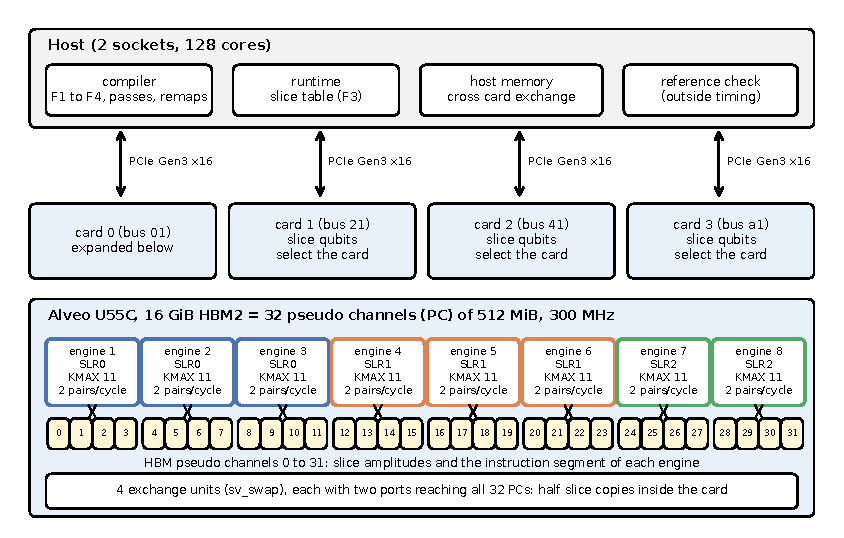
\includegraphics[width=\linewidth]{figures/fig_architecture.pdf}
\caption{Data flow of the engine on four cards. Local, slice controlled (F2) and slice diagonal (F1) gates
run in the HBM passes of every engine; slice relabelling (F3) changes only the slice table on the host; remaps
exchange half slices inside a card (device copy) or across cards (PCIe and host memory).}\label{fig:architecture}
\end{figure}
\section{Host Runtime and Distributed Protocol}\label{sec:host}

\subsection{Baseline design: three barrier exchange}\label{subsec:exchange}

In the baseline design one host process per card drives the card's kernel; the processes share three
\texttt{multiprocessing.Barrier} objects $B_A$, $B_B$, $B_C$ and a read buffer $R[j]$ and write buffer $W[j]$ per card in
shared host memory. A gate on partition qubits that is not diagonal is executed in three phases: each card reads its
slice from HBM into $R[j]$ and waits at $B_A$; each card computes its new slice from the slices of its partner cards in
NumPy, writes it to $W[j]$ and waits at $B_B$; each card writes $W[j]$ back to HBM and waits at $B_C$. Algorithm~\ref{alg:exchange}
shows the Hadamard gate on partition qubit $q_p$. The card whose partition bit is one holds the amplitudes with
$b_{q_p}=1$, so its new amplitudes are $(R[j'] - \alpha^{(j)})/\sqrt{2}$, with the partner's amplitude first.

\begin{algorithm}[t]
\caption{Three barrier exchange for $H$ on partition qubit $q_p$ (card $j$, baseline design).}\label{alg:exchange}
\begin{algorithmic}[1]
\Require partition bit index $p_b = q_p - n_\ell$, local slice $\alpha^{(j)}$
\State $R[j] \gets$ slice read from HBM \Comment{$2^{n_\ell}$ amplitudes over PCIe}
\State wait at $B_A$
\State $b \gets (j \shr p_b) \band 1$;\quad $j' \gets j \oplus (1 \shl p_b)$
\If{$b = 0$}
  \State $W[j] \gets (\alpha^{(j)} + R[j'])/\sqrt{2}$
\Else
  \State $W[j] \gets (R[j'] - \alpha^{(j)})/\sqrt{2}$
\EndIf
\State wait at $B_B$
\State write $W[j]$ to HBM \Comment{$2^{n_\ell}$ amplitudes over PCIe}
\State wait at $B_C$
\end{algorithmic}
\end{algorithm}

Every gate that touches a partition qubit therefore moves the whole slice of every card over PCIe twice: the exchange
path for the exchange, and the diagonal path because the phase is multiplied on the host. Table~\ref{tab:bytes} reports
the measured bytes per gate class.

\subsection{Engine runtime}\label{subsec:runtime}

The engine runtime drives all engines of all cards from one host process. For each segment it uploads the
instruction stream to every slice buffer, starts every engine of every card with its logical slice index, and waits
for all of them; cards run concurrently. A slice relabelling (F3) only updates the table that maps buffers to logical
slices. A remap swaps half slices: when both partner slices are on the same card and the moving chunks are large, the
card's exchange kernel copies them inside HBM; otherwise the moving halves are read over PCIe into host memory, swapped
there and written back, with one transfer per buffer when the chunks are small. The runtime records the time and the
bytes of every phase (Table~\ref{tab:timing}).

\subsection{Compilation flow}\label{subsec:compilation}

Every benchmark circuit is built once by \texttt{bench/circuits.py} (fixed seeds) and passed unchanged to the FPGA
engines and to the Qiskit CPU runs of Section~\ref{subsec:res-cpu}; QASM copies are part of the reproduction package.
The flow from a Qiskit circuit to engine records has five steps, all on the host and all included in
$T_{\mathrm{compile}}$ (Table~\ref{tab:timing}):
\begin{enumerate}
\item \emph{Gate intake.} Gates of one or two qubits are taken as unitary matrices from Qiskit
(\texttt{Operator}); multi controlled $X$, $Z$ and phase gates are taken directly as one controlled $2\times2$
operation. Such a gate stays one record as long as its target and its local controls fit the tile window and its
other controls sit on slice qubits, where the slice enable (F2) applies them; with $k$ tile qubits and $s$ slice qubits
this allows gates of up to $k+s$ qubits. Wider gates, every gate wider than the tile window when F2 is switched off,
and gates without a controlled form are decomposed by the Qiskit transpiler with \texttt{basis\_gates=[u, cx]},
\texttt{optimization\_level=1}. No other transpilation is applied, so the
FPGA and CPU runs see the same gate sequence.
\item \emph{Fusion and relabelling.} Runs of single qubit gates on one qubit are multiplied into one matrix; SWAP
gates are absorbed into the logical to physical qubit map and cost nothing.
\item \emph{Classification.} With the current qubit map each operation is classified as local, slice controlled
(F2), slice diagonal (F1), slice permutation (F3) or exchange (Section~\ref{subsec:engine}).
\item \emph{Scheduling.} Operations are appended to the current pass while their qubits fit the tile window;
an exchange operation first triggers a remap that brings its slice qubit to a local position, choosing as victims the
local qubits used furthest in the future, and the remapped qubit stays local for all later gates on it. A multi controlled gate wider than the tile window is placed by one remap that swaps its target with one of
its own controls, which then acts through the slice enable, and moves surplus local controls to free slice positions;
this keeps the Grover oracle a single record up to $n=14$ on one and two cards and $n=16$ on four cards.
\item \emph{Encoding.} Passes between remaps form one segment, uploaded once to every engine and executed by one
launch per engine.
\end{enumerate}

In a statevector simulator the cost is set by the number of full sweeps over the state and by the amplitudes that
cross slices, not by circuit depth. GHZ preparation, a serial chain of CX gates, shows what this means for the
compilation. On the engine all CX gates of the textbook GHZ chain whose qubits are local
share one pass, so depth does not cost sweeps; what costs is each CX whose target is a slice qubit, because the
target must first be brought into the slice (one remap per slice qubit, \NumGhzChainRemapsNoFfour~remaps with four
cards and \NumEnginesFlagship~engines per card). A logarithmic depth construction~\cite{cruz2019efficient} reduces depth but
leaves this count almost unchanged (\NumGhzLogRemapsNoFfour). The compiler therefore applies a hardware specific
rewrite (F4): for an $X$ type gate (CX, Toffoli) whose target is a slice qubit and whose controls are local, it moves
the controls up into slice positions instead of moving the target down. The remap costs the same, but the gate and
every later CX among these qubits then become slice relabelling (F3) or slice controlled (F2) operations; the GHZ
chain needs \NumGhzChainRemapsFfour~remap at every width. Because the rewrite can also increase traffic (it does for
the controlled modular multipliers of Shor's circuit), the compiler schedules every circuit with and without F4 and
keeps the schedule with fewer remaps. Section~\ref{subsec:res-ablation} reports the measured times of all variants.
\section{Benchmark Circuits}\label{sec:algorithms}

All circuits are produced by one generator with fixed seeds; their gate counts and routing are generated from the
compiler counters and reported in Table~\ref{tab:routing}.

\paragraph{Quantum Fourier transform.} The $n$ qubit QFT consists of $n$ Hadamard gates, $n(n-1)/2$ controlled phase
gates $\mathrm{CP}(\pi/2^{j-i})$ and $\lfloor n/2\rfloor$ final SWAP gates, a total of $n(n+1)/2 + \lfloor n/2\rfloor$
gates~\cite{nielsen2010quantum}. In the baseline design with the two top qubits as partition qubits, the routing of
the QFT at $n=12$ is 59 local, 21 diagonal and 4 exchange gates (the two Hadamard gates on the partition qubits and the
two SWAP gates that cross the partition boundary), counted gate by gate on the circuit before lowering. On the engine
SWAP gates are relabellings and the counts of Table~\ref{tab:routing} apply. The QFT is also run on a Haar random input state and as a round trip (a random
product state, QFT, inverse QFT), whose output equals its input.

\paragraph{GHZ and Bell states.} The GHZ state is prepared by the textbook chain (H on qubit 0 and CX$(i,i+1)$), by a
fan out from the top qubit, and by the logarithmic depth construction of Cruz et al.~\cite{cruz2019efficient};
the Bell state is H on qubit 0 followed by CX from qubit 0 to qubit $n-1$.

\paragraph{Grover search.} For one marked state among $N = 2^n$ and $\theta = \arcsin(2^{-n/2})$, $k$ iterations give
the success probability $P(k) = \sin^2\bigl((2k+1)\theta\bigr)$. We use the standard iteration count
$k_{\mathrm{opt}} = \lfloor \pi/(4\theta) \rfloor$, which lies next to the first maximum of $P(k)$ and guarantees
$P(k_{\mathrm{opt}}) \ge 1 - 2^{-n}$~\cite{boyer1998tight,grover1996fast}; because $P(k)$ is periodic in $k$, larger
iteration counts can come closer to one, at several times the cost. All Grover runs use $k_{\mathrm{opt}}$, and we
report the measured target probability against $P(k_{\mathrm{opt}})$; for $n=4$ this probability is 0.9613. The oracle
and diffuser use one multi controlled $X$ gate each, which the engine executes as a single record.

\paragraph{Phase estimation (Shor).} The order finding component of Shor's algorithm~\cite{shor1997polynomial} is
run as quantum phase estimation of the modular multiplication by $a = 7$ modulo $N = 15$ (order $r = 4$) with a
counting register of $t$ qubits and four work qubits; the counting register must show four peaks of probability $1/4$
at multiples of $2^t/4$. To scale the phase estimation to the full width we also run it on the phase gate $P(2\pi\phi)$
with $\phi = 5/16$, whose $t$ qubit counting register must return $2^t\phi$ with probability one. A larger order
finding instance (for example $N = 21$) needs modular multipliers that we did not implement; the phase estimation on
the phase gate covers the same circuit structure at every width.

\paragraph{Random and worst case circuits.} Random circuits have layers of random U3 gates on every qubit and CX or
CZ gates on random disjoint pairs. The worst case for the distributed design applies H and RX gates to the top qubits
in every layer, so that every layer contains non diagonal gates on partition qubits.
\section{Methodology}\label{sec:methodology}

\subsection{What the reported times contain}\label{subsec:timing}

Every phase is timed on the host with \texttt{time.perf\_counter} and recorded per run; Table~\ref{tab:timing} lists
the phases and states which of them each reported time includes. Device open and bitstream load ($T_{\mathrm{setup}}$)
happen once per session and are reported separately. $T_{\mathrm{e2e}}$ is the time from the Qiskit circuit object to
the sampled measurement results (1024 shots) and includes compilation, all transfers, all kernel time, all exchanges,
the final read back and sampling; it excludes $T_{\mathrm{setup}}$ and the reference computation used for fidelity.
For the baseline design the same boundaries are used; its worker processes are started once per session.

\begin{table}[t]
\caption{Timing phases and their inclusion in the reported times.}\label{tab:timing}
\begin{tabular}{@{}llcc@{}}
\toprule
Phase & Contents & in $T_{\mathrm{e2e}}$ & in $T_{\mathrm{kernel}}$ \\
\midrule
$T_{\mathrm{setup}}$ & device open, bitstream load, worker start (once per session) & no & no \\
$T_{\mathrm{compile}}$ & Qiskit circuit to engine records (both F4 schedules) & yes & no \\
$T_{\mathrm{h2d}}$ & initial state on the device, instruction uploads & yes & no \\
$T_{\mathrm{kernel}}$ & all engine launches, start to completion of the last engine & yes & yes \\
$T_{\mathrm{exch}}$ & remaps: device copies, host exchanges (PCIe and host copy), relabelling & yes & no \\
$T_{\mathrm{d2h}}$ & final read back of all slices & yes & no \\
$T_{\mathrm{post}}$ & sampling of 1024 shots from the slices & yes & no \\
reference & Qiskit or Aer reference state and error metrics & no & no \\
\bottomrule
\end{tabular}
\end{table}

\subsection{Protocol}\label{subsec:protocol}

Each configuration runs one warm up repetition, which is discarded, followed by \NumRepsMin\ to \NumRepsMax~timed
repetitions (more for short runs, fewer for the widest runs, whose length is bounded by the thermal limit of
Section~\ref{sec:limitations}). We report the median and the interquartile range.
Runs were made with no other job on the host (no build, no other benchmark; checked and logged before every campaign).
The CPU frequency governor was \NumGovernor\ and is recorded with every campaign. All circuits come from one
generator with fixed seeds (Section~\ref{subsec:compilation}); random input states are drawn from the Haar measure with
a fixed seed per width.

\subsection{Correctness metrics}\label{subsec:metrics}

For every reported instance the final state $\psi$ (read back from HBM, outside the timed region) is compared with
an independent reference $\psi_{\mathrm{ref}}$: the Qiskit \texttt{Statevector} class for $n \le \NumRefSvMax$ and Qiskit
Aer in double precision with gate fusion disabled above. We report the fidelity
$F = |\langle \psi_{\mathrm{ref}} | \psi \rangle|^2$, the infidelity computed without cancellation as
$1 - F = d^2 - d^4/4$ with $d = \min_\phi \lVert \psi - e^{i\phi} \psi_{\mathrm{ref}} \rVert$ for normalised states, the
largest amplitude error after optimal global phase alignment, and the $\ell_2$ error $d$. A global phase is
physically irrelevant and is removed by the alignment; it is nonetheless reported, since the baseline design's gate
decompositions drop global phases. Grover runs additionally report the measured target probability against the
analytic value $\sin^2((2k+1)\theta)$, and the phase estimation runs the full distribution of the counting register.

\subsection{CPU reference timing}\label{subsec:method-cpu}

To compare the FPGA simulation time with the Qiskit simulation time, on the same host and
for exactly the same circuit objects we time (i) the Qiskit \texttt{Statevector} class (NumPy, complex128, one
thread) and (ii) Qiskit Aer, statevector method, double precision, with its default thread count and with one
thread (versions in Table~\ref{tab:platform}). For Aer the circuit is transpiled to the simulator's native gate set
with \texttt{optimization\_level=0}, which keeps multi controlled gates such as the Grover oracle as single gates, and
Aer's default gate fusion is left enabled, as a user would run it; the reference states for correctness are computed
with fusion disabled. The FPGA engine receives the same circuit object and compiles a multi controlled gate into
one record (Section~\ref{subsec:compilation}); the baseline design lowers it to its 19 opcodes with the decomposition
of its original code. Only the simulation call is timed; circuit construction and transpilation
are excluded for both CPU and FPGA, and the FPGA time we compare against is $T_{\mathrm{e2e}}$, which does include the
FPGA side compilation. A comparison with GPU simulators is not repeated here: a detailed FPGA, CPU and CUDA-Q GPU
comparison on the same type of card is the subject of the companion single card study~\cite{tiwari2026fpga30}, and this
paper makes no speed claim against GPU simulators.

\subsection{Energy}\label{subsec:method-energy}

Board power of each card is read from its management controller (sum of the 12~V PCIe, 12~V auxiliary and 3.3~V rails,
the quantity reported by \texttt{xbutil}) every 0.1~s during a dedicated energy stage, in which every configuration is
repeated several times. The controller refreshes its readings about once per second. For every run the board power of a
card is the time weighted mean of the readings in force during the run, including the reading taken before the run
started, and the energy is this power times the end to end time, summed over the cards in use; we report the median
over the repetitions together with the number of new readings that fell inside the shortest run (Table~\ref{tab:energy}).
Host CPU and memory power are not measured, because the RAPL energy counters of this host are readable only with
administrator rights, so the energy figures cover the accelerator boards only.
\section{Results}\label{sec:results}

\subsection{Correctness}\label{subsec:res-correctness}

Table~\ref{tab:correctness} summarises the comparison of every reported instance with the independent reference
(Section~\ref{subsec:metrics}). All \NumCorrectnessInstances~checked instances, from $n=\NumCorrectnessNmin$ to
$n=\NumCorrectnessNmax$ on one, two and four cards, \NumCorrectnessHaar~of them from Haar random input states, agree with the
reference to double precision rounding: the largest amplitude error is \NumWorstMaxAbsErr\ and the largest infidelity
$1-F$ is \NumWorstOneMinusF. In \NumCorrectnessExact~instances the state is bit identical to the reference. The engine keeps every gate matrix in
float64; the baseline design transfers gate angles as float32 and widens them in the kernel. Its largest amplitude
error is \NumBaselineExactErrMax\ for QFT, GHZ and Bell states from $\ket{0\dots0}$, where no rotation angle affects the
result (in the QFT every controlled phase acts while its control qubit is still $\ket{0}$), but \NumBaselineRotErrMax\ for
random circuits, Grover search and Haar random inputs, whose rotations change the state. Grover search with $k_{\mathrm{opt}}$ iterations
(Table~\ref{tab:grover}) reaches the analytic target probability $\sin^2((2k_{\mathrm{opt}}+1)\theta)$ to within
\NumGroverWorstPdiff. The counting registers of the phase estimation runs (order finding for $N=15$ and phase estimation
of $P(2\pi\phi)$, rows shor15 and qpe of Table~\ref{tab:correctness}) reproduce the probability distribution of the
reference to within \NumQpeWorstDistDiff~in every outcome.

\begin{table}[t]
\caption{Correctness of the engine: worst values over all instances of each circuit family, after optimal
global phase alignment. Instances: every width and card count of the campaign; zero input $\ket{0\dots0}$ or Haar random.}\label{tab:correctness}
\begin{tabular}{@{}llcrrrr@{}}
\toprule
Circuit & Input & $n$ & Instances & max $1-F$ & max $|\Delta\alpha|$ & max $\ell_2$ \\
\midrule
bell & zero & 4 to 22 & 10 & $1.23\times 10^{-32}$ & $1.11\times 10^{-16}$ & $1.11\times 10^{-16}$ \\
ghz & haar & 8 to 28 & 11 & $3.88\times 10^{-32}$ & $1.40\times 10^{-17}$ & $1.97\times 10^{-16}$ \\
ghz & zero & 4 to 31 & 28 & $1.23\times 10^{-32}$ & $1.11\times 10^{-16}$ & $1.11\times 10^{-16}$ \\
grover & zero & 4 to 16 & 7 & $8.07\times 10^{-25}$ & $1.04\times 10^{-14}$ & $8.98\times 10^{-13}$ \\
partition heavy & haar & 8 to 28 & 11 & $8.50\times 10^{-31}$ & $7.93\times 10^{-17}$ & $9.22\times 10^{-16}$ \\
partition heavy & zero & 4 to 22 & 10 & $4.19\times 10^{-31}$ & $3.72\times 10^{-16}$ & $6.47\times 10^{-16}$ \\
qft & haar & 8 to 28 & 11 & $1.08\times 10^{-30}$ & $6.40\times 10^{-17}$ & $1.04\times 10^{-15}$ \\
qft & zero & 4 to 31 & 24 & $4.57\times 10^{-30}$ & $8.67\times 10^{-19}$ & $2.14\times 10^{-15}$ \\
qft iqft & zero & 4 to 28 & 13 & $2.57\times 10^{-30}$ & $3.33\times 10^{-16}$ & $1.60\times 10^{-15}$ \\
qpe & zero & 12 to 28 & 10 & $1.31\times 10^{-25}$ & $2.00\times 10^{-13}$ & $3.62\times 10^{-13}$ \\
rand10 & haar & 12 to 28 & 10 & $3.83\times 10^{-30}$ & $6.14\times 10^{-17}$ & $1.96\times 10^{-15}$ \\
rand10 & zero & 4 to 28 & 13 & $3.67\times 10^{-30}$ & $2.39\times 10^{-16}$ & $1.92\times 10^{-15}$ \\
shor15 & zero & 12 to 24 & 8 & $5.84\times 10^{-30}$ & $1.16\times 10^{-15}$ & $2.42\times 10^{-15}$ \\
\bottomrule
\end{tabular}
\end{table}

\begin{table}[t]
\caption{Grover search with $k_{\mathrm{opt}}$ iterations on four cards: measured target probability against
$P(k_{\mathrm{opt}}) = \sin^2((2k_{\mathrm{opt}}+1)\theta)$.}\label{tab:grover}
\begin{tabular}{@{}rrrrr@{}}
\toprule
$n$ & $k_{\mathrm{opt}}$ & $P(k)$ analytic & $P$ measured & difference \\
\midrule
4 & 3 & 0.961319 & 0.961319 & $7.66\times 10^{-15}$ \\
6 & 6 & 0.996586 & 0.996586 & $1.87\times 10^{-14}$ \\
8 & 12 & 0.999947 & 0.999947 & $4.55\times 10^{-14}$ \\
10 & 25 & 0.999461 & 0.999461 & $1.11\times 10^{-13}$ \\
12 & 50 & 0.999945 & 0.999945 & $2.55\times 10^{-13}$ \\
14 & 100 & 1.000000 & 1.000000 & $5.80\times 10^{-13}$ \\
16 & 201 & 0.999988 & 0.999988 & $1.31\times 10^{-12}$ \\
\bottomrule
\end{tabular}
\end{table}

\subsection{Largest simulated width}\label{subsec:res-maxwidth}

\begin{table}[t]
\caption{Largest width verified against the reference per number of cards and circuit, HBM occupied per card by the
state, end to end time (median of the timed repetitions; n/a for the single validation runs) and the largest amplitude
error.}\label{tab:maxwidth}
\begin{tabular}{@{}rlrrrr@{}}
\toprule
Cards & Circuit & largest $n$ & HBM per card (GiB) & $T_{\mathrm{e2e}}$ (s) & max $|\Delta\alpha|$ \\
\midrule
1 & ghz & 29 & 8 & n/a & $1.11\times 10^{-16}$ \\
1 & qft & 29 & 8 & n/a & $1.02\times 10^{-19}$ \\
1 & rand10 & 28 & 4 & 21.9 & $6.10\times 10^{-19}$ \\
2 & ghz & 30 & 8 & n/a & $1.11\times 10^{-16}$ \\
2 & qft & 30 & 8 & n/a & $7.12\times 10^{-20}$ \\
2 & rand10 & 28 & 2 & n/a & $5.22\times 10^{-19}$ \\
4 & ghz & 31 & 8 & 13.7 & $1.11\times 10^{-16}$ \\
4 & qft & 31 & 8 & 60.8 & $5.42\times 10^{-20}$ \\
4 & qft iqft & 28 & 1 & 20.8 & $7.38\times 10^{-17}$ \\
4 & rand10 & 29 & 2 & 31.1 & $4.16\times 10^{-19}$ \\
\bottomrule
\end{tabular}
\end{table}

\begin{table}[t]
\caption{Instances stopped by the thermal guard (a card reached 90\,\textdegree C FPGA or 85\,\textdegree C HBM): setting of
the slice paths, completed repetitions, the card and its temperatures at the stop. The paths column gives F1, F2, F3 and
F4 in this order (1 on, 0 off, a: F4 chosen by the compiler, Section~\ref{subsec:compilation}).}\label{tab:thermal}
\begin{tabular}{@{}rlrlrrr@{}}
\toprule
Cards & Circuit & $n$ & paths & repetitions & card & FPGA / HBM (C) \\
\midrule
4 & qft & 28 & 0000 & 4 of 6 & 21 & 90 / 85 \\
4 & rand10 & 8 & 111a & 1 of 3 & 21 & 93 / 88 \\
4 & grover & 16 & 111a & 5 of 6 & 21 & 90 / 85 \\
4 & qft iqft & 24 & 111a & 0 of 6 & 21 & 90 / 85 \\
4 & qft & 31 & 111a & 2 of 2 & 21 & 91 / 86 \\
4 & qft & 30 & 111a & 3 of 4 & 21 & 90 / 85 \\
4 & ghz & 31 & 111a & 0 of 1 & 21 & 90 / 85 \\
\bottomrule
\end{tabular}
\end{table}

The capacity follows from the memory layout. Every HBM buffer of a slice lies in one pseudo channel of 512~MiB and
holds the slice together with the engine's instruction segment of 4~MiB. For the widest states each card has
\NumPcsUsedFlagship~slices, one per PC, of at most $2^{24}$ amplitudes (256~MiB), so one card holds $n=29$, two cards
$n=30$ and four cards $n=31$. The verified widths reach this capacity on every configuration: \NumMaxWidthOneCard,
\NumMaxWidthTwoCards~and \NumMaxWidthFourCards~qubits (Table~\ref{tab:maxwidth}). The state then takes 8~GiB of the
16~GiB of each card, spread over all 32 pseudo channels. The next power of two, $2^{25}$ amplitudes, would fill a pseudo
channel completely and leave no room for the instruction segment that shares the buffer, so the engine reaches every
pseudo channel but fills only half of the HBM (Section~\ref{sec:limitations}). At $n=31$ GHZ
preparation and the QFT run on the four cards in \NumMaxThirtyOneGhzS~s and \NumMaxThirtyOneQftS~s and agree with the
reference computed by Qiskit Aer. Earlier attempts at this width were stopped by the thermal guard of one card
(Table~\ref{tab:thermal}).

\subsection{FPGA resources}\label{subsec:res-resources}

Table~\ref{tab:resources} gives the post route utilisation of both bitstreams. The baseline kernel occupies
\NumLutPctVsix\,\% of the LUTs, \NumDspPctVsix\,\% of the DSPs and \NumBramPctVsix\,\% of the BRAM and closes timing at
\NumClockVsix~MHz. The engine build with \NumEnginesFlagship~compute units uses \NumLutPctFlagship\,\% of the LUTs,
\NumDspPctFlagship\,\% of the DSPs, \NumBramPctFlagship\,\% of the BRAM tiles and \NumUramPctFlagship\,\% of the URAM at \NumClockFlagship~MHz. The DSPs
implement the double precision arithmetic of the $2\times2$ primitive. The build with sixteen compute units placed but
failed in routing (Section~\ref{subsec:engine}), so the engine count is limited by routing congestion rather than by the
number of LUTs or DSPs. The PC bindings of both builds are
given in Sections~\ref{subsec:baseline-design} and~\ref{subsec:engine}.

\begin{table}[t]
\caption{Post route utilisation (full device including the shell) and achieved kernel clock of the bitstreams
used in this paper.}\label{tab:resources}
\begin{tabular}{@{}lrrrrrr@{}}
\toprule
Build & MHz & LUT (\%) & FF (\%) & DSP (\%) & BRAM tiles (\%) & URAM (\%) \\
\midrule
baseline (8 data ports) & 258 & 209{,}980 (16.1) & 250{,}174 (9.6) & 727 (8.1) & 238 (11.8) & 0 (0.0) \\
engine, 8 compute units & 300 & 486{,}506 (37.3) & 684{,}497 (26.2) & 2{,}692 (29.8) & 808 (40.1) & 64 (6.7) \\
engine, 16 compute units & \multicolumn{6}{l}{placed; routing failed (conflicted nets)} \\
device total (XCU55C) & & 1{,}303{,}680 & 2{,}607{,}360 & 9{,}024 & 2{,}016 & 960 \\
\bottomrule
\end{tabular}
\end{table}

\subsection{Where the time goes}\label{subsec:res-breakdown}

\begin{table}[t]
\caption{Routing of the engine on four cards (compiler counters). ``gates'' counts the gates of the circuit; the
following columns count operations after fusion of consecutive single qubit gates and absorption of SWAP gates into the
qubit map, so they do not add up to the gate count: local operations, partition controlled (F2), partition diagonal (F1),
slice relabelling (F3) and operations that required a remap; then remaps and HBM passes.}\label{tab:routing}
\begin{tabular}{@{}lrrrrrrrrr@{}}
\toprule
Circuit & $n$ & gates & local & F2 & F1 & F3 & exchange & remaps & passes \\
\midrule
bell & 20 & 2 & 1 & 0 & 0 & 0 & 1 & 1 & 2 \\
ghz & 20 & 20 & 15 & 1 & 0 & 3 & 1 & 1 & 4 \\
ghz & 28 & 28 & 23 & 1 & 0 & 3 & 1 & 1 & 6 \\
partition heavy & 20 & 40 & 15 & 0 & 0 & 0 & 2 & 2 & 2 \\
qft & 20 & 220 & 116 & 55 & 31 & 0 & 8 & 8 & 24 \\
qft & 28 & 420 & 268 & 85 & 44 & 0 & 9 & 9 & 76 \\
qft iqft & 20 & 460 & 258 & 153 & 6 & 0 & 21 & 21 & 59 \\
qft iqft & 28 & 868 & 563 & 244 & 8 & 0 & 23 & 23 & 169 \\
rand10 & 20 & 300 & 279 & 0 & 0 & 0 & 21 & 21 & 29 \\
rand10 & 28 & 420 & 400 & 0 & 0 & 0 & 20 & 20 & 46 \\
\bottomrule
\end{tabular}
\end{table}

\begin{figure}[t]
\centering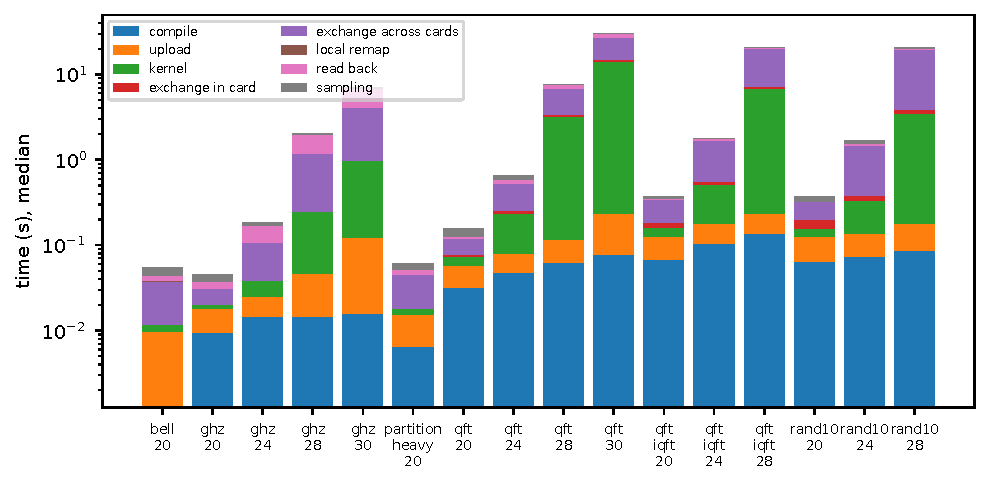
\includegraphics[width=\linewidth]{figures/fig_breakdown.pdf}
\caption{Per phase time of the engine on four cards (median of the timed repetitions).}\label{fig:breakdown}
\end{figure}

\begin{table}[t]
\caption{Baseline design on four cards: routing, bytes moved over PCIe and share of the run time per
phase (slowest card).}\label{tab:bytes}
\begin{tabular}{@{}lrrrrrrrrr@{}}
\toprule
Circuit & $n$ & local & diag. & exch. & PCIe (MiB) & kernel \% & PCIe \% & host \% & sync \% \\
\midrule
bell & 8 & 1 & 0 & 1 & 0.0 & 6 & 32 & 3 & 58 \\
bell & 14 & 1 & 0 & 1 & 1.0 & 19 & 26 & 5 & 50 \\
bell & 22 & 1 & 0 & 1 & 256.0 & 52 & 17 & 17 & 13 \\
ghz & 8 & 6 & 0 & 2 & 0.0 & 7 & 26 & 5 & 62 \\
ghz & 14 & 12 & 0 & 2 & 1.5 & 39 & 5 & 25 & 31 \\
ghz & 22 & 20 & 0 & 2 & 384.0 & 94 & 2 & 2 & 2 \\
partition heavy & 8 & 0 & 0 & 40 & 0.3 & 0 & 31 & 5 & 64 \\
partition heavy & 14 & 0 & 0 & 40 & 20.5 & 0 & 35 & 7 & 58 \\
partition heavy & 22 & 0 & 0 & 40 & 5248.0 & 0 & 48 & 26 & 27 \\
qft & 8 & 23 & 13 & 4 & 0.1 & 12 & 32 & 3 & 54 \\
qft & 14 & 83 & 25 & 4 & 15.0 & 88 & 5 & 1 & 7 \\
qft & 22 & 219 & 41 & 4 & 5888.0 & 98 & 1 & 0 & 1 \\
qft & 26 & 311 & 49 & 4 & 110592.0 & 98 & 0 & 0 & 1 \\
qft iqft & 8 & 52 & 26 & 10 & 0.3 & 11 & 31 & 4 & 54 \\
qft iqft & 14 & 178 & 50 & 10 & 30.5 & 89 & 5 & 1 & 6 \\
qft iqft & 22 & 458 & 82 & 10 & 11904.0 & 98 & 1 & 0 & 1 \\
rand10 & 8 & 81 & 10 & 29 & 0.3 & 8 & 26 & 4 & 61 \\
rand10 & 14 & 171 & 11 & 28 & 20.0 & 64 & 9 & 7 & 19 \\
rand10 & 22 & 290 & 14 & 26 & 5248.0 & 94 & 2 & 1 & 2 \\
\bottomrule
\end{tabular}
\end{table}

\begin{figure}[t]
\centering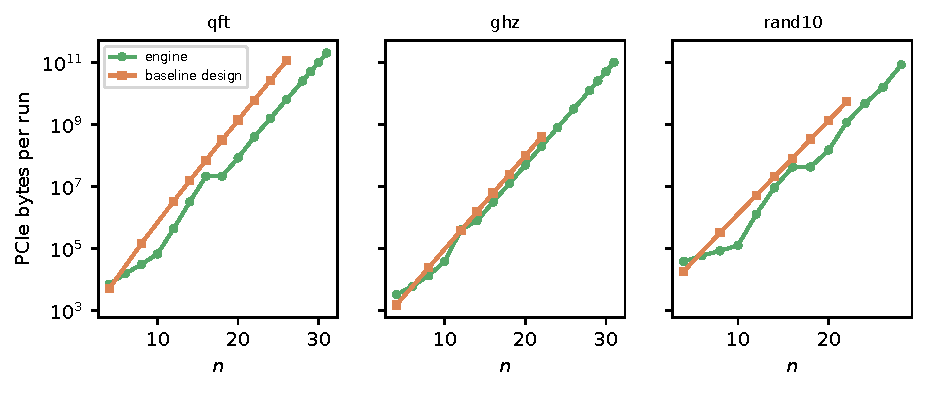
\includegraphics[width=\linewidth]{figures/fig_bytes.pdf}
\caption{PCIe bytes per run on four cards, including the state upload and read back, for the baseline design and
the engine (the engine also counts its instruction uploads).}\label{fig:bytes}
\end{figure}

\begin{table}[t]
\caption{Engine microbenchmarks on four cards, \NumEnginesFlagship~engines per card: launch of an empty segment, one
pass with one operation, and the HBM rate it implies (one read and one write of every slice), for slice widths $L$.}\label{tab:micro}
\begin{tabular}{@{}rrrrrr@{}}
\toprule
$L$ & slice (MiB) & launch (ms) & one pass (ms) & HBM, all cards (GB/s) & per card (GB/s) \\
\midrule
11 & 0.03125 & 0.79 & 0.78 & 3 & 1 \\
12 & 0.0625 & 0.79 & 0.781 & 5 & 1 \\
13 & 0.125 & 0.78 & 0.52 & 16 & 4 \\
14 & 0.25 & 1.06 & 0.593 & 28 & 7 \\
15 & 0.5 & 0.79 & 0.609 & 55 & 14 \\
16 & 1 & 0.77 & 0.689 & 97 & 24 \\
17 & 2 & 1.01 & 0.922 & 146 & 36 \\
18 & 4 & 0.77 & 1.21 & 221 & 55 \\
19 & 8 & 0.77 & 2.19 & 245 & 61 \\
20 & 16 & 0.79 & 3.61 & 298 & 74 \\
21 & 32 & 0.76 & 6.55 & 328 & 82 \\
22 & 64 & 0.83 & 12.2 & 353 & 88 \\
23 & 128 & 0.82 & 23.2 & 370 & 92 \\
24 & 256 & 1.00 & 45.3 & 379 & 95 \\
\bottomrule
\end{tabular}
\end{table}

\paragraph{HBM streaming and compute.} A pass reads and writes every slice once. With slices of $2^{\NumHbmLmax}$
amplitudes the \NumEnginesFlagship~engines of each card stream \NumHbmPerCard~GB/s per card, \NumHbmAllCards~GB/s on four
cards (Table~\ref{tab:micro}); this is the measured rate of the design, well below the 460~GB/s peak of the
HBM~\cite{amd_ds978}, and small slices are dominated by the launch time of \NumLaunchMs~ms. When a pass carries more
operations the engine becomes compute bound: each additional operation at $L=\NumPassmL$ costs \NumOpCostMs~ms, close to
the \NumOpCostModelMs~ms that follow from two amplitude pairs per cycle at \NumClockFlagship~MHz.

\paragraph{Engine.} Table~\ref{tab:routing} shows where the gates go. Of the \NumRouteQftGates~gates of the
QFT at $n=28$, \NumRouteQftLocal~run locally, \NumRouteQftFtwo~under the slice enable (F2) and \NumRouteQftFone~as slice
diagonal records (F1); the SWAP gates are absorbed into the qubit map, and only \NumRouteQftExch~gates need a remap. The
records are packed into \NumRouteQftPasses~HBM passes, so the state is swept far fewer times than there are gates. On four
cards the FPGA kernels then take \NumQftTwentyEightKernelPct\,\% of the end to end time and PCIe transfers (state
upload, exchanges across cards, read back) \NumQftTwentyEightPciePct\,\% (Fig.~\ref{fig:breakdown}); the remaining time
is compilation and host bookkeeping. The exchanges are thus the part that more cards make larger
(Section~\ref{subsec:res-scaling}).

\paragraph{Baseline design.} Table~\ref{tab:bytes} gives the same breakdown for the baseline design. For small
circuits most of its time is synchronisation of the card processes: \NumVsixQftEightSyncPct\,\% for the QFT at $n=8$,
against \NumVsixQftEightKernelPct\,\% in the kernel. From $n\approx 14$ on, its per gate kernel sweeps dominate, with
\NumVsixQftTwentyTwoKernelPct\,\% of the time at $n=22$, which is the behaviour modelled in Section~\ref{subsec:res-model}.
A circuit whose gates all act on partition qubits never reaches the kernel: the partition heavy circuit at $n=22$ spends
\NumVsixPhTwentyTwoPciePct\,\% in PCIe transfers, \NumVsixPhTwentyTwoHostPct\,\% in host arithmetic and
\NumVsixPhTwentyTwoSyncPct\,\% in synchronisation. These are the two costs that the engine removes: per gate
sweeps by packing records into passes, and host arithmetic by executing partition gates on the cards.

\subsection{Scaling over one, two and four cards}\label{subsec:res-scaling}

\begin{table}[t]
\caption{End to end time $T$ (median), speedup $S = T_1/T_C$ and parallel efficiency $E = S/C$ for $C$ cards.}\label{tab:scaling}
\begin{tabular}{@{}lrrrrrrrr@{}}
\toprule
 & & 1 card & \multicolumn{3}{c}{2 cards} & \multicolumn{3}{c}{4 cards} \\
\cmidrule(lr){3-3}\cmidrule(lr){4-6}\cmidrule(l){7-9}
Circuit & $n$ & $T$ (s) & $T$ (s) & $S$ & $E$ (\%) & $T$ (s) & $S$ & $E$ (\%) \\
\midrule
ghz & 20 & 0.0255 & 0.0397 & 0.64 & 32 & 0.0464 & 0.55 & 14 \\
ghz & 22 & 0.0425 & 0.0573 & 0.74 & 37 & 0.0746 & 0.57 & 14 \\
ghz & 24 & 0.132 & 0.176 & 0.75 & 37 & 0.17 & 0.77 & 19 \\
ghz & 26 & 0.458 & 0.576 & 0.79 & 40 & 0.55 & 0.83 & 21 \\
ghz & 28 & 1.64 & 2.09 & 0.79 & 39 & 1.97 & 0.84 & 21 \\
qft & 20 & 0.104 & 0.109 & 0.95 & 47 & 0.154 & 0.67 & 17 \\
qft & 22 & 0.243 & 0.217 & 1.12 & 56 & 0.282 & 0.86 & 22 \\
qft & 24 & 0.8 & 0.578 & 1.38 & 69 & 0.676 & 1.18 & 30 \\
qft & 26 & 3.26 & 2.08 & 1.56 & 78 & 2.1 & 1.55 & 39 \\
qft & 27 & 6.72 & 4.19 & 1.60 & 80 & n/a & &  \\
qft & 28 & 13.8 & 8.49 & 1.62 & 81 & 7.77 & 1.77 & 44 \\
rand10 & 20 & 0.17 & 0.221 & 0.77 & 38 & 0.373 & 0.46 & 11 \\
rand10 & 22 & 0.4 & 0.408 & 0.98 & 49 & 0.611 & 0.65 & 16 \\
rand10 & 24 & 1.22 & 1.23 & 0.98 & 49 & 1.54 & 0.79 & 20 \\
rand10 & 26 & 4.05 & 5.1 & 0.80 & 40 & 4.79 & 0.85 & 21 \\
rand10 & 27 & 8.23 & 6.39 & 1.29 & 64 & n/a & &  \\
rand10 & 28 & 21.9 & 18.4 & 1.19 & 60 & 19.7 & 1.11 & 28 \\
\bottomrule
\end{tabular}
\end{table}

\begin{figure}[t]
\centering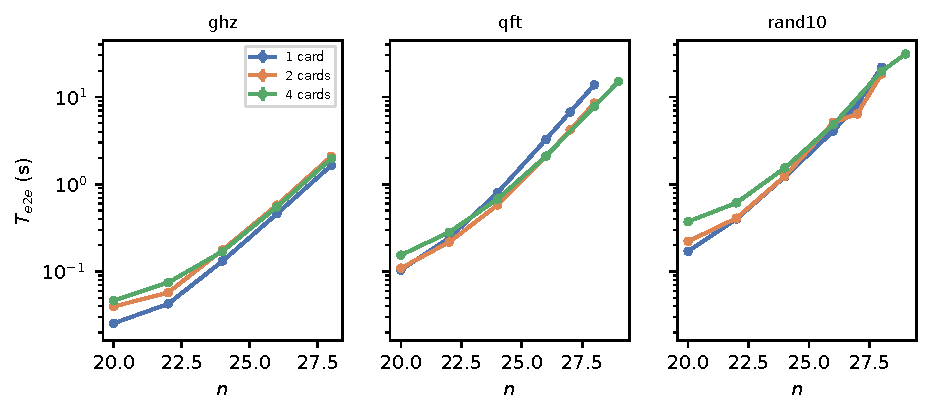
\includegraphics[width=\linewidth]{figures/fig_scaling.pdf}
\caption{End to end time on one, two and four cards (median, whiskers: interquartile range).}\label{fig:scaling}
\end{figure}

Distribution over more cards buys capacity, not speed (Table~\ref{tab:scaling}, Fig.~\ref{fig:scaling}). In
\NumScaleBelowOne~of \NumScaleCases~comparisons the two or four card run is slower than the one card run of the same
circuit. The best case is the QFT at $n=\NumScaleBestFourN$, with a speedup of \NumQftTwentyEightSpeedupTwo~on two and
\NumScaleBestFour~on four cards. The reason is the exchange path. On one card all slices share one HBM, and remaps run as
device copies, except for large remaps whose device copy chunks would be too small, which the runtime moves through host
memory. With more cards the top qubits become card qubits, and every remap that involves one of them crosses PCIe through
host memory, because peer to peer transfers between the cards are not available on this host
(Section~\ref{sec:limitations}). For the QFT at $n=28$ the exchanges take \NumScaleExchQftOne\,\% of the end to end
time on one card and \NumScaleExchQftFour\,\% on four cards, of which \NumScaleExchHostQftFour~s through the host; for the
random circuit they grow from \NumScaleExchRandOne\,\% to \NumScaleExchRandFour\,\%. The more cards hold the state,
the more of the run is PCIe traffic; with the present exchange path the four card system is the way to simulate
$n=30$ and $n=31$, not a way to simulate $n\le 29$ faster than one card. With the same number of amplitudes per card (weak scaling, $n$ on one card against $n+2$ on four), separate runs
of the QFT and the random circuit at $n=26$ and 27 on one card against $n=28$ and 29 on four cards (the four card runs
at $n=29$ are not part of Table~\ref{tab:scaling}) reach a weak scaling efficiency $T_1(n)/T_4(n+2)$ of
\NumWeakEffFourMin\,\% to \NumWeakEffFourMax\,\%, highest for the QFT and lowest for the random circuit, for the same
reason.

\subsection{Ablation of the slice paths and of the compiler rewrite}\label{subsec:res-ablation}

\begin{table}[t]
\caption{Slice paths switched off one at a time and together on two and four cards ($C$), at the largest width of the
ablation: end to end time (median) and number of remaps with all paths on and all off.}\label{tab:ablation}
\begin{tabular}{@{}lrrrrrrrrrr@{}}
\toprule
 & & & \multicolumn{6}{c}{$T_{\mathrm{e2e}}$ (s)} & \multicolumn{2}{c}{remaps} \\
\cmidrule(lr){4-9}\cmidrule(l){10-11}
Circuit & $C$ & $n$ & all on & F1 off & F2 off & F3 off & F4 off & all off & on & off \\
\midrule
qft & 2 & 28 & 8.53 & 9.63 & 50.5 & 8.55 & 8.5 & 54.1 & 8 & 98 \\
qft & 4 & 28 & 7.92 & 10 & 73 & 8.04 & 8.04 & 83.2 & 9 & 119 \\
ghz & 2 & 28 & 2.05 & 2.03 & 3.63 & 5.62 & 5.7 & 5.73 & 1 & 4 \\
ghz & 4 & 28 & 1.95 & 2.04 & 3.72 & 7.98 & 7.85 & 7.92 & 1 & 5 \\
rand10 & 2 & 28 & 18.4 & 18.2 & 18.5 & 18.3 & 18.2 & 18.3 & 16 & 16 \\
rand10 & 4 & 28 & 20.7 & 20.5 & 20.5 & 20.5 & 20.5 & 20.4 & 20 & 20 \\
partition heavy & 2 & 28 & 2.51 & 2.57 & 2.57 & 2.57 & 2.51 & 2.45 & 2 & 2 \\
partition heavy & 4 & 28 & 2.64 & 2.67 & 2.66 & 2.66 & 2.72 & 2.68 & 2 & 2 \\
grover & 2 & 14 & 2.56 & 2.73 & 279 & 2.27 & 2.34 & 151 & 803 & 10004 \\
grover & 4 & 14 & 2.8 & 2.85 & 285 & 2.39 & 2.08 & 156 & 803 & 10004 \\
\bottomrule
\end{tabular}
\end{table}

\begin{table}[t]
\caption{Baseline design, QFT on four cards with and without the partition diagonal path (the diagonal gates then
take the exchange path): routing, execution time, host compute and barrier time (slowest card), PCIe bytes of all cards,
and the speedup of the diagonal path (medians).}\label{tab:diag}
\begin{tabular}{@{}rlrrrrrrr@{}}
\toprule
$n$ & diagonal path & diagonal & exchanges & $T_{\mathrm{exec}}$ (s) & host compute (s) & barriers (s) & PCIe (MiB) & speedup \\
\midrule
8 & on & 13 & 4 & 0.0356 & 0.00118 & 0.0026 & 0 & 1.11 \\
 & off & 0 & 17 & 0.0394 & 0.0021 & 0.00743 & 0 &  \\
12 & on & 21 & 4 & 0.156 & 0.00194 & 0.00345 & 3 & 1.07 \\
 & off & 0 & 25 & 0.166 & 0.00403 & 0.0146 & 3 &  \\
16 & on & 29 & 4 & 3.58 & 0.0933 & 0.077 & 68 & 1.13 \\
 & off & 0 & 33 & 4.03 & 0.338 & 0.314 & 68 &  \\
18 & on & 33 & 4 & 18 & 0.136 & 0.0847 & 304 & 1.02 \\
 & off & 0 & 37 & 18.3 & 0.375 & 0.269 & 304 &  \\
20 & on & 37 & 4 & 89.9 & 0.336 & 0.119 & 1344 & 1.01 \\
 & off & 0 & 41 & 91.3 & 0.954 & 0.931 & 1344 &  \\
\bottomrule
\end{tabular}
\end{table}

\begin{figure}[t]
\centering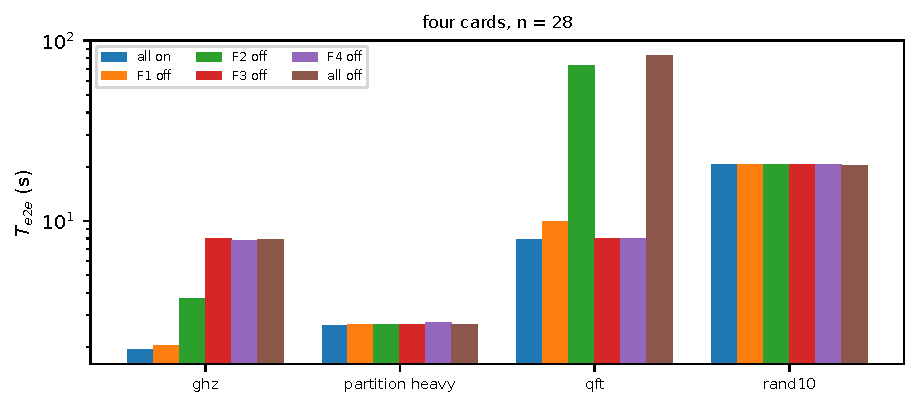
\includegraphics[width=\linewidth]{figures/fig_ablation.pdf}
\caption{End to end time of the engine on four cards with the slice paths switched off one at a time and
together, at the largest ablation width.}\label{fig:ablation}
\end{figure}

\paragraph{GHZ preparation and the compiler rewrite F4.} Three GHZ constructions were run on four cards with F4 off
and on (Section~\ref{subsec:compilation}). Without F4 the CX chain needs one remap per slice qubit,
\NumGhzChainRemapsNoFfour~at every width, and the logarithmic depth construction~\cite{cruz2019efficient} needs the same
number (\NumGhzLogRemapsNoFfour): a shorter circuit does not move fewer amplitudes. With F4 the chain needs
\NumGhzChainRemapsFfourAll~remap and the remaining CX gates become slice relabelling; at $n=28$ its end to end time falls
from \NumGhzChainTimeNoFfour~s to \NumGhzChainTimeFfour~s, a factor of \NumGhzChainSpeedupFfour~(Table~\ref{tab:ablation},
F4 off against all on). The chain rooted at the
top qubit improves by a factor of \NumGhzTopSpeedupFfour~(\NumGhzTopRemapsFfourAll~remaps), while the logarithmic
construction keeps \NumGhzLogRemapsFfourAll~remaps, because its CX targets are spread over the register. For this
hardware the useful optimisation of GHZ preparation is therefore the placement of the controls, not the depth of the
circuit.

\paragraph{Slice paths.} Table~\ref{tab:ablation} switches the slice paths off one at a time and together; a gate
whose path is off falls back to a remap. For the QFT on two cards at $n=28$ the slice controlled path F2 carries almost
the whole benefit: without it the run is \NumAblQftTwoFtwoOff~times slower, with all paths off \NumAblQftTwoAllOff~times.
Its controlled phase gates on partition qubits have a local target and a slice control, which F2 applies under the slice
enable; the slice diagonal path F1, used when the target itself is a slice qubit, adds a factor of \NumAblQftTwoFoneOff.
GHZ preparation relies on slice relabelling and the control promotion (F3, F4) and becomes \NumAblGhzTwoAllOff~times
slower without the slice paths. Grover search at $n=\NumAblGroverTwoN$ depends most on F2: its multi controlled
gates stay single records only with the slice enable (Section~\ref{subsec:compilation}); without F2 they are decomposed,
and the run is \NumAblGroverTwoFtwoOff~times slower, \NumAblGroverTwoAllOff~times with all paths off. The random circuits and the partition heavy circuit are unaffected
(\NumAblRandTwoAllOff~and \NumAblPhTwoAllOff): their slice qubits carry non diagonal single qubit gates (the random
U3 layers; H and RX in the partition heavy circuit), which need a remap with or without the slice paths, and once a slice
qubit is local the following gates on it run locally. For circuits dominated by non diagonal gates on partition
qubits the exchange path therefore sets the time. On four cards, where more gates touch slice qubits, the effects are larger: the QFT is
\NumAblQftFourFtwoOff~times slower without F2 and \NumAblQftFourAllOff~times with all paths off, GHZ
\NumAblGhzFourAllOff~times, and Grover search \NumAblGroverFourFtwoOff~times without F2.

\paragraph{Diagonal path of the baseline design.} In the baseline design a diagonal gate on a partition qubit avoids
the exchange between cards but still moves the slice of every card to the host and back, so the PCIe traffic is the
same with and without the diagonal path (\NumDiagPcieTwenty~MiB for the QFT at $n=20$, Table~\ref{tab:diag}). The path
saves host arithmetic (\NumDiagHostOffTwenty~s against \NumDiagHostOnTwenty~s at $n=20$) and barrier time
(\NumDiagBarrierOffTwenty~s against \NumDiagBarrierOnTwenty~s), but the run is dominated by the kernel sweeps of the local
gates, and the speedup of the diagonal path is only \NumDiagSpeedupMin~to \NumDiagSpeedupMax. Executing diagonal and
controlled gates on partition qubits pays off only when they run on the cards, as in the engine, where switching these
paths off makes the QFT \NumAblQftFourAllOff~times slower on four cards.

\begin{table}[t]
\caption{Choice of the partition qubits: the top qubits select the card (default) or qubits 0 and 1 do. End to end
time (median), remaps, and the ratio of the two times.}\label{tab:part}
\begin{tabular}{@{}lrrrrrrr@{}}
\toprule
 & & & \multicolumn{2}{c}{top qubits} & \multicolumn{2}{c}{qubits 0 and 1} & \\
\cmidrule(lr){4-5}\cmidrule(lr){6-7}
Circuit & $n$ & $C$ & $T_{\mathrm{e2e}}$ (s) & remaps & $T_{\mathrm{e2e}}$ (s) & remaps & ratio \\
\midrule
ghz & 16 & 2 & 0.0258 & 1 & 0.0186 & 3 & 0.72 \\
ghz & 16 & 4 & 0.0336 & 1 & 0.0581 & 4 & 1.73 \\
ghz & 20 & 2 & 0.0259 & 1 & 0.0236 & 3 & 0.91 \\
ghz & 20 & 4 & 0.0349 & 1 & 0.042 & 3 & 1.21 \\
ghz & 24 & 2 & 0.158 & 1 & 0.109 & 3 & 0.69 \\
ghz & 24 & 4 & 0.15 & 1 & 0.16 & 3 & 1.07 \\
grover & 8 & 2 & 0.0389 & 0 & 0.0372 & 1 & 0.96 \\
grover & 8 & 4 & 0.0388 & 0 & 0.0514 & 3 & 1.32 \\
grover & 12 & 2 & 0.398 & 201 & 0.401 & 201 & 1.01 \\
grover & 12 & 4 & 0.567 & 201 & 0.817 & 303 & 1.44 \\
grover & 14 & 2 & 2.62 & 803 & 3.15 & 804 & 1.20 \\
grover & 14 & 4 & 2.73 & 803 & 2.98 & 804 & 1.09 \\
qft & 16 & 2 & 0.0499 & 5 & 0.0524 & 5 & 1.05 \\
qft & 16 & 4 & 0.126 & 10 & 0.103 & 8 & 0.82 \\
qft & 20 & 2 & 0.11 & 7 & 0.105 & 6 & 0.95 \\
qft & 20 & 4 & 0.156 & 8 & 0.16 & 7 & 1.03 \\
qft & 24 & 2 & 0.576 & 8 & 0.745 & 6 & 1.29 \\
qft & 24 & 4 & 0.655 & 9 & 0.649 & 8 & 0.99 \\
\bottomrule
\end{tabular}
\end{table}

Assigning the card to qubits 0 and 1 instead of the top qubits changes the end to end time by a factor between
\NumPartRatioMin~and \NumPartRatioMax~(Table~\ref{tab:part}), and no choice is better for every circuit. The QFT acts on
all qubits alike and is nearly indifferent. GHZ needs more remaps with the low partition, because its CX chain starts at
qubit 0, yet on two cards it runs faster: all its remaps then involve engine qubits inside a card and run as device
copies, while with the top partition one remap crosses the cards through host memory. On four cards one remap still
crosses the cards, and the low partition is slower.
Grover search changes little because its oracle spans the whole register in either case. The top qubit partition is
therefore kept as the default, and the runtime accepts any initial placement.

\subsection{Comparison with Qiskit on the same host}\label{subsec:res-cpu}

\begin{table}[t]
\caption{End to end time of the FPGA system (four cards) and simulation time of Qiskit on the host CPU for the same
circuits (medians, seconds).}\label{tab:cpu}
\begin{tabular}{@{}lrrrrrr@{}}
\toprule
Circuit & $n$ & FPGA $T_{\mathrm{e2e}}$ & Statevector & Aer (all threads) & Aer (1 thread) & FPGA/Aer \\
\midrule
ghz & 12 & 0.011 & 0.000908 & 0.00172 & 0.00143 & 6.4 \\
ghz & 16 & 0.0326 & 0.0255 & 0.15 & 0.00762 & 0.22 \\
ghz & 20 & 0.0447 & 0.295 & 0.00459 & 0.135 & 9.7 \\
ghz & 22 & 0.0702 & 1.21 & 0.213 & 0.641 & 0.33 \\
ghz & 24 & 0.181 & 4.38 & 0.0867 & 2.81 & 2.1 \\
ghz & 26 & 0.555 & n/a & 0.349 & 12.2 & 1.6 \\
ghz & 28 & 2.02 & n/a & 1.31 & 52.4 & 1.5 \\
ghz & 30 & 6.98 & n/a & 5.23 & 251 & 1.3 \\
grover & 4 & 0.00854 & 0.00302 & 0.00143 & 0.00132 & 6 \\
grover & 6 & 0.0194 & 0.483 & 0.00477 & 0.00426 & 4.1 \\
grover & 8 & 0.0413 & 1.93 & 0.00681 & 0.00677 & 6.1 \\
grover & 10 & 0.0864 & 7.24 & 0.0226 & 0.0224 & 3.8 \\
grover & 12 & 0.55 & 23.8 & 0.0708 & 0.0711 & 7.8 \\
grover & 14 & 2.73 & 283 & 0.376 & 0.375 & 7.2 \\
grover & 16 & 22.7 & n/a & 0.644 & 1.66 & 35 \\
qft & 12 & 0.0216 & 0.00707 & 0.00572 & 0.00573 & 3.8 \\
qft & 16 & 0.12 & 0.554 & 0.0144 & 0.0301 & 8.3 \\
qft & 20 & 0.157 & 4.08 & 0.0296 & 0.514 & 5.3 \\
qft & 22 & 0.282 & 15.9 & 0.0654 & 2.4 & 4.3 \\
qft & 24 & 0.66 & 62.9 & 0.211 & 11.2 & 3.1 \\
qft & 26 & 2.06 & n/a & 0.88 & 50.2 & 2.3 \\
qft & 28 & 7.63 & n/a & 3.82 & 233 & 2 \\
qft & 30 & 30 & n/a & 17 & 1.15e+03 & 1.8 \\
qft iqft & 12 & 0.0392 & 0.0148 & 0.0166 & 0.0163 & 2.4 \\
qft iqft & 16 & 0.232 & 0.528 & 0.0351 & 0.0601 & 6.6 \\
qft iqft & 20 & 0.368 & 8.25 & 0.0539 & 1.07 & 6.8 \\
qft iqft & 22 & 0.589 & 33 & 0.114 & 4.98 & 5.2 \\
qft iqft & 24 & 1.8 & 131 & 0.392 & 22.8 & 4.6 \\
qft iqft & 26 & 6.3 & n/a & 1.84 & 104 & 3.4 \\
qft iqft & 28 & 20.8 & n/a & 7.21 & 481 & 2.9 \\
rand10 & 12 & 0.0495 & 0.0118 & 0.0109 & 0.0114 & 4.5 \\
rand10 & 16 & 0.275 & 0.379 & 0.0131 & 0.0401 & 21 \\
rand10 & 20 & 0.371 & 4.83 & 0.0286 & 0.696 & 13 \\
rand10 & 22 & 0.608 & 18.6 & 0.066 & 2.95 & 9.2 \\
rand10 & 24 & 1.66 & 70.3 & 0.368 & 13.7 & 4.5 \\
rand10 & 26 & 4.87 & n/a & 1.04 & 57.2 & 4.7 \\
rand10 & 28 & 20.5 & n/a & 4.38 & 252 & 4.7 \\
\bottomrule
\end{tabular}
\end{table}

\begin{figure}[t]
\centering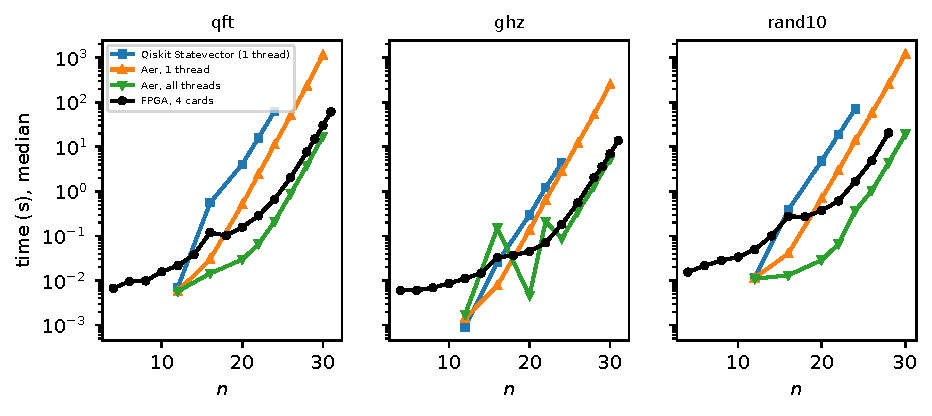
\includegraphics[width=\linewidth]{figures/fig_cpu.pdf}
\caption{End to end time of the FPGA system on four cards against Qiskit on the same host (median).}\label{fig:cpu}
\end{figure}

Qiskit Aer with all hardware threads of the \NumHostCores~core host is faster than the four card system for
almost every circuit and width (Table~\ref{tab:cpu}, Fig.~\ref{fig:cpu}): the FPGA system is faster in
\NumCpuFpgaFaster~of \NumCpuCases~cases, both GHZ circuits at widths where the multithreaded Aer time is irregular.
The gap narrows with the width, because the fixed costs of the FPGA system (compilation, launches, transfers) are
amortised and its time is set by HBM passes and exchanges: for the QFT the FPGA system is \NumCpuRatioQftSixteen~times
slower than Aer at $n=16$ and \NumCpuRatioQft~times slower at $n=30$; for GHZ at $n=30$ the factor is \NumCpuRatioGhz.
Against a single CPU thread the FPGA system is faster in \NumCpuFasterThanAerOne~of \NumCpuAerOneCases~cases and by
\NumCpuAerOneOverQft~times for the QFT at $n=30$. Grover search is the least favourable case: each iteration contains two
multi controlled gates over the whole register, which bring different qubits into the cards in turn, so that at $n=16$
the \NumGroverSixteenIters~iterations need \NumGroverSixteenRemaps~remaps, the exchanges take \NumGroverSixteenExchPct\,\%
of the end to end time, and the four card system is \NumCpuRatioGroverSixteen~times slower than Aer. We therefore make no claim of speed advantage over a multithreaded CPU
simulator on this host; the comparison with GPUs on the same card type is in the companion paper~\cite{tiwari2026fpga30}.

\subsection{Dependence on the host}\label{subsec:res-host}

\begin{table}[t]
\caption{End to end time (median, seconds) with the host process and its workers restricted to the first $N$ hardware
threads (logical CPUs $0$ to $N-1$) of the \NumHostCores~core, \NumHostThreads~thread host.}\label{tab:host}
\begin{tabular}{@{}lrlrrrrrr@{}}
\toprule
 & & & & \multicolumn{5}{c}{hardware threads} \\
\cmidrule(l){5-9}
Design & $C$ & Circuit & $n$ & 4 & 8 & 16 & 64 & 256 \\
\midrule
baseline & 4 & qft & 16 & 3.59 & 3.53 & 3.54 & 3.58 & 3.55 \\
baseline & 4 & qft & 20 & 90.3 & 89.1 & 89.2 & 89.3 & 89.2 \\
engine & 2 & qft & 20 & 0.108 & 0.108 & 0.11 & 0.111 & 0.109 \\
engine & 2 & qft & 24 & 0.594 & 0.598 & 0.594 & 0.591 & 0.568 \\
engine & 2 & rand10 & 20 & 0.213 & 0.215 & 0.229 & 0.223 & 0.19 \\
engine & 2 & rand10 & 24 & 1.29 & 1.32 & 1.29 & 1.28 & 1.22 \\
engine & 4 & qft & 20 & 0.149 & 0.147 & 0.151 & 0.154 & 0.142 \\
engine & 4 & qft & 24 & 0.683 & 0.667 & 0.67 & 0.665 & 0.644 \\
engine & 4 & rand10 & 20 & 0.35 & 0.354 & 0.372 & 0.369 & 0.353 \\
engine & 4 & rand10 & 24 & 1.6 & 1.62 & 1.59 & 1.6 & 1.61 \\
\bottomrule
\end{tabular}
\end{table}

Restricting the engine runtime to between \NumHostCoresMin~and \NumHostCoresMax~hardware threads changes its end to
end time by at most \NumHostSpreadEnginePct\,\% on two and four cards, without a trend over the number of cores; the
largest spreads belong to runs of a few tenths of a second (Table~\ref{tab:host}). The runtime is one process whose
work is compilation, launches and transfers, and the gate arithmetic runs on the cards. The \NumHostCores~cores of our
host are therefore not needed: \NumHostCoresMin~hardware threads give the same times. A smaller host still needs one PCIe slot per
card and host memory for the exchanged half slices; other hosts were not measured.
The baseline design varies by \NumHostSpreadBaselinePct\,\% under the same restriction: its QFT time is spent
in the kernel sweeps of Section~\ref{subsec:res-model}, and its host arithmetic for the gates on partition qubits is a
small part of the run.

\subsection{A model of the baseline design}\label{subsec:res-model}

\begin{table}[t]
\caption{Baseline design, QFT on four cards: routing counters, measured execution time (median) and the time
predicted from microbenchmarks alone (no fitted parameter).}\label{tab:model}
\begin{tabular}{@{}rrrrrrrr@{}}
\toprule
$n$ & sweeps & launches & slice transfers & measured (s) & model (s) & model/measured & sweeps (\%) \\
\midrule
4 & 9 & 2 & 9 & 0.0179 & n/a & n/a & n/a \\
8 & 123 & 7 & 17 & 0.0345 & 0.0219 & 0.63 & 3 \\
12 & 349 & 2 & 25 & 0.155 & 0.148 & 0.96 & 82 \\
14 & 504 & 13 & 29 & 0.692 & 0.74 & 1.07 & 94 \\
16 & 687 & 15 & 33 & 3.5 & 3.82 & 1.09 & 98 \\
18 & 898 & 17 & 37 & 17.8 & 19.5 & 1.09 & 99 \\
20 & 1137 & 19 & 41 & 89.2 & 97.5 & 1.09 & 100 \\
22 & 1404 & 21 & 45 & 440 & 480 & 1.09 & 100 \\
24 & 1699 & 23 & 49 & 2.13e+03 & 2.32e+03 & 1.09 & 100 \\
26 & 2022 & 25 & 53 & 1.02e+04 & 1.11e+04 & 1.08 & 100 \\
\bottomrule
\end{tabular}
\end{table}

\begin{figure}[t]
\centering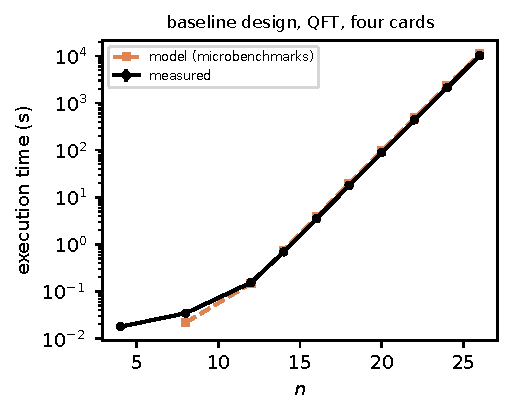
\includegraphics[width=0.6\linewidth]{figures/fig_model.pdf}
\caption{Baseline design, QFT on four cards: measured execution time and the microbenchmark model.}\label{fig:model}
\end{figure}

The timing curve of the baseline design is nearly flat for small widths and then turns upward. To explain the bend, the model of Table~\ref{tab:model}
uses only microbenchmarks of the baseline kernel on the same cards
(one launch, one gate, collection and distribution of a slice, command round trip and barrier) and the native operation
counts of each circuit, obtained by replaying the routing and the lowering of the baseline host (and checked against
the counters recorded on the cards); the relative cost of single qubit, CX and CZ operations follows from the loop
bounds and initiation intervals of the kernel source. No parameter is fitted to the circuit timings. For $n\ge 12$ the
model predicts the measured QFT time to within a factor of \NumModelRatioMin~to \NumModelRatioMax~(Fig.~\ref{fig:model}).
The QFT at $n=20$ on four cards appears in several campaigns of the baseline design (Tables~\ref{tab:model},
\ref{tab:diag} and~\ref{tab:host}); the values differ by the variation between campaigns and by whether the execution
time or the end to end time is quoted, and every comparison in the text takes both of its values from the same campaign.

The bend has a simple origin. The baseline kernel sweeps the whole slice for every native operation, and the time of a
sweep doubles with every qubit: \NumVsixSweepMsTen~ms for a slice of $2^{10}$ amplitudes and \NumVsixSweepMsSixteen~ms for
$2^{16}$, i.e.\ $t_0 = \NumVsixNsPerAmp$~ns per amplitude, or \NumVsixCyclesPerAmp~cycles of the
\NumClockVsix~MHz kernel clock. The fixed costs do not grow with the width up to slices of about $2^{14}$ amplitudes: a
kernel launch (\NumVsixLaunchMsTen~ms), the transfer of a slice to the host and back (\NumVsixXferMsTen~ms at
$2^{10}$ amplitudes), a command round trip between the host processes (\NumQueueRttUs~$\mu$s) and a barrier
(\NumBarrierUs~$\mu$s); they are set by PCIe, the XRT runtime and the host. With $W$ weighted native operations,
$N_L$ launches, $N_X$ slice transfers and $N_E$ exchanges (Table~\ref{tab:model}), the model reads
\begin{equation}
T(n) \approx W\,t_0\,2^{n_\ell} + N_L\,(t_L + t_q) + N_X\,(t_X + t_q) + 3N_E\,t_b, \qquad n_\ell = n - \log_2 C,
\label{eq:model}
\end{equation}
and the bend lies where the first term equals the sum of the others,
\begin{equation}
n^\ast = \log_2 C + \log_2 \frac{N_L\,(t_L + t_q) + N_X\,(t_X + t_q) + 3N_E\,t_b}{W\,t_0}.
\label{eq:bend}
\end{equation}
With the counts of the QFT for $n=8$ to 16 on four cards, Eq.~\eqref{eq:bend} gives $n^\ast$ between
\NumModelNstarMin~and \NumModelNstarMax. The measured runs agree: the sweeps take \NumModelSweepShareEight\,\% of the model
time at $n=8$ and more than half from $n=\NumModelCrossN$ on, after which the curve follows the exponential growth of the
sweeps, multiplied by the number of native operations, which grows with $n$ as well. The bend is therefore set by the
ratio of the per amplitude sweep time of the kernel to the fixed costs of PCIe and the host, both measured on the
platform; a faster kernel (smaller $t_0$) moves it to larger $n$, a faster host path to smaller $n$.

\subsection{Energy}\label{subsec:res-energy}

\begin{table}[t]
\caption{Board energy per simulation: time weighted mean of the board power of every used card (XMC sensors, about
one reading per second) times the end to end time. The last column is the smallest number of sensor readings
inside one run.}\label{tab:energy}
\begin{tabular}{@{}lrrrrrr@{}}
\toprule
Circuit & $n$ & $C$ & $T_{\mathrm{e2e}}$ (s) & board power (W) & energy (J) & readings \\
\midrule
qft & 26 & 1 & 3.27 & 34.3 & 112 & 1 \\
qft & 26 & 2 & 2.16 & 68.2 & 147 & 0 \\
qft & 26 & 4 & 2.12 & 136.6 & 290 & 0 \\
qft & 28 & 1 & 13.8 & 35.0 & 482 & 4 \\
qft & 28 & 2 & 8.49 & 68.3 & 580 & 1 \\
qft & 28 & 4 & 7.82 & 137.1 & 1.07e+03 & 1 \\
rand10 & 26 & 1 & 4.11 & 45.3 & 186 & 3 \\
rand10 & 26 & 2 & 5.22 & 76.4 & 399 & 3 \\
rand10 & 26 & 4 & 4.53 & 144.7 & 655 & 1 \\
rand10 & 28 & 1 & 21.9 & 41.1 & 901 & 8 \\
rand10 & 28 & 2 & 18.4 & 77.4 & 1.42e+03 & 5 \\
rand10 & 28 & 4 & 20.2 & 141.5 & 2.86e+03 & 3 \\
\bottomrule
\end{tabular}
\end{table}

During the simulations the four cards draw together between \NumEnergyPowerMinFour~and \NumEnergyPowerMaxFour~W of
board power (Table~\ref{tab:energy}). The lowest readings of the same stage, taken while the cards wait parked
between runs, add up to \NumEnergyIdleFour~W, so about two thirds of the power is static, and the energy of a
simulation follows its run time: a QFT at $n=28$ on four cards takes \NumEnergyQftTwentyEightFour~J. The card sensors
refresh about once per second, so for runs of a few seconds the power is the time weighted mean of the readings in force during the run (zero to three new ones);
the table gives the number of readings inside the shortest run. Host power is not included because the CPU energy
counters of this host are readable only with administrator rights. Since the power grows with every card and the run time does not fall in proportion
(Section~\ref{subsec:res-scaling}), the energy of a simulation rises with the number of cards: the QFT at $n=28$
takes \NumEnergyQftTwentyEightOne~J on one card, \NumEnergyQftTwentyEightTwo~J on two and
\NumEnergyQftTwentyEightFour~J on four. For widths that fit one card, one card is the most energy efficient
configuration of this system.
\section{Discussion}\label{sec:discussion}

\paragraph{What the engine changes.} The baseline design keeps every gate on a partition qubit on the host and sweeps
the whole slice once per native operation. Its run time is therefore set by per gate kernel sweeps for wide circuits
and by synchronisation for small ones, as the model of Section~\ref{subsec:res-model} shows without any fitted
parameter. The engine removes both costs: gates that need no amplitudes of another slice run on the cards under
the slice enable (F1 to F3), consecutive records share one HBM pass, and the state uses all 32 pseudo channels of each
card. The QFT at $n=20$ on four cards takes \NumHostSubmittedQftTwenty~s in the baseline design and
\NumHostRevisedQftTwenty~s in the engine on the same cards, \NumSubmittedOverRevisedQftTwenty~times less.

\paragraph{Where the system stands.} We make no claim of speed advantage. Qiskit Aer with all threads of the host is
faster than the four card system for almost every circuit of Table~\ref{tab:cpu}; the FPGA system is faster than a
single CPU thread in all \NumCpuWideCases~cases with $n\ge 24$, and its time approaches that of the multithreaded CPU as
the width grows. Our measured HBM rate, \NumHbmPerCard~GB/s per card, is well below the peak of the memory, and the engine is compute bound
when a pass carries several operations; a design that issues more amplitude pairs per cycle, or more engines than the
eight that routed in complex128, would raise the rate of the cards. The comparison with GPUs on the same card type is in
the companion paper~\cite{tiwari2026fpga30}.

\paragraph{What distribution buys.} Each doubling of the cards adds one qubit of capacity in complex128, from 29 qubits on
one card to 31 on four (Section~\ref{subsec:res-maxwidth}; verified: \NumMaxWidthOneCard, \NumMaxWidthTwoCards~and
\NumMaxWidthFourCards~qubits), at the price of exchanges through host memory. Scaling and energy show the price:
more cards make most runs slower and every run more energy hungry (Sections~\ref{subsec:res-scaling}
and~\ref{subsec:res-energy}). The slice paths and the compiler rewrite keep the exchanges to a minimum where the circuit
allows it: without them the QFT on four cards is \NumAblQftFourAllOff~times slower and GHZ preparation
\NumAblGhzFourAllOff~times. Circuits whose slice qubits carry general gates, such as random circuits, gain nothing from
them and pay the full exchange cost.

\paragraph{Relation to other multi device simulators.} Distributed CPU and GPU simulators use the same global to local
swap and reach far larger widths on many nodes~\cite{haner2017petabyte,deraedt2019massively,imamura2022mpiqulacs}. The
Trefoil system distributes much larger states over FPGAs with SATA storage, trading bandwidth for
capacity~\cite{niwase2023trefoil,wei2025qutrefoil}. The present design keeps the state in HBM, which limits the width to
the memory of the cards but keeps every pass at HBM speed; its weak point is the exchange path between the cards, which
peer to peer transfers or direct card to card links would shorten.

\paragraph{Reproducibility.} Every number in this paper is generated by script from the raw measurement files, each of
which records the code commit, the bitstream hash and the cards used. The circuits, the transpilation settings, the
timing definitions and the measurement protocol are given in Section~\ref{sec:methodology}, and the raw data are
available as stated in the declarations.
\section{Limitations}\label{sec:limitations}

\paragraph{Thermal limit of one card.} The four cards sit in one host with a shared air path, and the card at PCIe
bus 21 runs hottest. With the engine bitstream loaded, that card heats above 84\,\textdegree C within minutes even
when no kernel runs. Every measurement therefore runs under a guard: before each repetition, a card at 85\,\textdegree C
(FPGA) or 80\,\textdegree C (HBM) is parked on the small bitstream of the baseline design and cooled below
84\,\textdegree C; a run during which a card reaches 90\,\textdegree C (FPGA) or 85\,\textdegree C (HBM) is kept,
flagged, and ends that configuration. Table~\ref{tab:thermal} lists the \NumThermalStops~configurations that the guard
stopped, all on card 21; where a stopped configuration was run again later, the complete run is the one reported. In one early attempt the cooling wait was done
with the engine bitstream still loaded; card 21 reached 96\,\textdegree C (FPGA) and 91\,\textdegree C (HBM), its AXI
firewall tripped and the driver reset the card. That run is excluded from all results and the procedure was changed
as described. The widest runs, at $n=31$ on four cards, succeeded only after cooling pauses; on this host the time
available for long runs at full width is limited by the temperature of one card, not by memory.

\paragraph{Routing limit of the engine count.} A build with sixteen complex128 engines did not route
(Section~\ref{sec:architecture}). The engine uses eight compute units with four pseudo channels each; it reaches
all 32 pseudo channels of a card, but the peak kernel throughput is that of eight engines.

\paragraph{Half of the HBM holds the state.} At full width the state occupies 8~GiB of the 16~GiB of each card
(Section~\ref{subsec:res-maxwidth}): every pseudo channel holds $2^{24}$ amplitudes (256~MiB) of a slice next to the
engine's instruction segment, which shares the buffer, and the next power of two would fill the 512~MiB channel
completely. Storing the instructions in a separate buffer, on a further HBM port or in on chip memory, would remove this
limit and give one more qubit per configuration ($n=30$ on one card, $n=32$ on four); we did not build this variant.

\paragraph{Data movement across cards goes through the host.} Gates that need amplitudes of another card are
executed after an exchange through host memory over PCIe. Peer to peer transfers between the cards are disabled on
this host (the platform reports that they would need 32~GB of PCIe address space per card), and we did not change that system
setting. The cost of this path for each circuit family is given in
Sections~\ref{subsec:res-scaling} and~\ref{subsec:res-ablation}. This path is why more cards do not make a run faster:
on four cards the exchanges take \NumScaleExchQftFour\,\% of the end to end time of the QFT at $n=28$ and
\NumScaleExchRandFour\,\% for the random circuit, and they set the time of every circuit whose slice qubits carry non
diagonal gates. Peer to peer transfers or a faster interconnect would shorten exactly this part.

\paragraph{Card count.} The partition assigns the top $\log_2 C$ qubits to the card index, so the number of cards
must be a power of two. The runtime accepts any such count, but only $C = 1$, 2 and 4 were run, because the host has
four cards. Eight cards would need a host with eight x16 slots, and every further card qubit adds remaps across cards
for the circuits that act on it; with the exchange through host memory, the trend of Section~\ref{subsec:res-scaling},
a growing exchange share with every doubling of the cards, would be expected to continue. We make no measured claim for
eight or more cards.

\paragraph{One host, one platform.} All measurements come from one host with four U55C cards. The behaviour of the
exchange on hosts with a different PCIe topology or with peer to peer transfers enabled was not measured.
\section{Conclusions}\label{sec:conclusions}

We presented a complex128 statevector engine for one, two and four AMD Alveo U55C cards and measured it, together with
a baseline design that computes the gates on partition qubits on the host, on four physical cards in one host. The engine executes every gate that needs no
amplitudes of another slice on the cards, including diagonal, slice controlled and slice permutation gates on partition
qubits and multi controlled gates wider than its tile, packs consecutive gates into HBM passes, and spreads the
state over all 32 pseudo channels of every card. It simulates \NumMaxWidthOneCard~qubits on one card, \NumMaxWidthTwoCards~on two and \NumMaxWidthFourCards~on four cards,
every instance agreeing with an independent reference to double precision rounding (largest amplitude error
\NumWorstMaxAbsErr). On the same cards the QFT at $n=20$ runs \NumSubmittedOverRevisedQftTwenty~times faster than in the
baseline design, whose timing curve a microbenchmark model without fitted parameters reproduces to within a factor
of \NumModelRatioMin~to \NumModelRatioMax.

The measurements also set the limits. Qiskit Aer on the \NumHostCores~core host is faster than the four card system for
almost all circuits measured. More cards add capacity but not speed, because remaps that involve a card qubit pass
through host memory: in \NumScaleBelowOne~of \NumScaleCases~comparisons two or four cards are slower than one, and the
energy of a simulation grows with the number of cards. One card of the host limits the widest runs thermally. The next
steps are therefore a faster exchange path between the cards, by peer to peer transfers or direct links, and a kernel
with a higher rate per card.

\backmatter

\bmhead{Acknowledgments}
This work was funded by the Ministry of Electronics and Information Technology (MeitY), Government of India. The
research was conducted at the C-DAC Noida Centre under the supervision of Mr. Abhishek Tiwari, Scientist F, Embedded
Systems Division, C-DAC Noida. We thank the developers of Qiskit and of the open FPGA tooling on which this study
depends.

\section*{Declarations}

\textbf{Funding.} This work was funded by the Ministry of Electronics and Information Technology (MeitY), Government of India.

\textbf{Conflict of interest.} The author declares no competing interests.

\textbf{Data availability.} The raw measurement records that support the findings of this study (one JSON file per
campaign with timestamps, code commit, bitstream hashes and card identifiers), the benchmark circuits in OpenQASM and
the scripts that generate every table and figure from them are available from the corresponding author on reasonable
request.

\textbf{Author contribution.} N.~Ali designed and implemented the HLS kernels, the host runtime and compiler and the
benchmark suite, carried out the measurements and wrote the manuscript.

\bibliography{references}

\end{document}
